%Préambule du document :
\documentclass[12pt, a4paper]{book}
%\usepackage[latin1]{inputenc} 
\usepackage[utf8]{inputenc} % accents
\usepackage{gensymb} % degree symbol ° (\degree)
\usepackage[T1]{fontenc} % | "`pipe"' character
\usepackage{graphicx}
\usepackage{titling}
\usepackage{amssymb} 
\usepackage{minitoc} % chapter's tocs
\usepackage{authblk} % author affiliations
\usepackage{fancyhdr} % modify the headers
\usepackage{tabularx} % tables not larger than A4
\usepackage[table]{xcolor} %colors inside the tables
\usepackage{float}
\usepackage{multicol} % multiple columns in some sections
\usepackage[inner=2cm,outer=2cm]{geometry} %A4 margins
\usepackage{siunitx}
\usepackage[labelfont=bf, margin=0.5cm]{caption} % for figure captions in minipages
\usepackage{hyperref} %link references (toc, citations) inside document
\usepackage{natbib} % to cite with parentheses and plain text et only year if you please...
\usepackage{amsmath}
 \usepackage{fixltx2e} % allows overrightarrow to be in caption
 \MakeRobust{\overrightarrow}




\bibliographystyle{plainnat} % reference style
\renewcommand{\bibname}{References} %Rename "`bibliography"' => "`references"'
\newcommand*{\doi}[1]{\href{https://doi.org/#1}{doi: #1}}

\hypersetup{
    colorlinks,
    citecolor=brown,
    filecolor=green,
    linkcolor=red,
    urlcolor=blue
}
\hypersetup{linktocpage}


\pagestyle{fancy}
\fancyhead{}
\fancyfoot{}
\fancyhead[RO,LE]{\thepage}
\fancyhead[LO]{\leftmark}
\fancyhead[RE]{\rightmark}
\setcounter{tocdepth}{1} % we only want chapters and sections in toc
\setcounter{minitocdepth}{2} %we want sections and subsections in chapters' minitocs

\pretitle{%
  \begin{center}
  \LARGE
  
\includegraphics[width=17cm]{Logo_software.png}\\[\bigskipamount]
}
\posttitle{\end{center}}

%\postdate{
%
\includegraphics[width=15cm]{logo_affiliations.png}
%}

\title{MorphoDig User's guide\\MorphoDig v1.3.0}



%\titlepicture[width=13cm]{Logo_software.png}
\author{Renaud LEBRUN}
\affil{Institut des Sciences de l'Evolution, University of Montpellier, France}
\date{\today} 


%Corps du document :
\begin{document}

	\dominitoc

\maketitle


\tableofcontents

\chapter*{Introduction}
\addstarredchapter{Introduction}

\markboth{INTRODUCTION}{}

\minitoc 

 MorphoDig is based on the design concepts of the software FoRM-IT (Fossil Reconstruction and Morphometry Interactive Toolkit; \citep{Zollikofer1995,Zollikofer2005}).
\ MorphoDig\citep{Lebrun2018} was developed as a help to the scientific journal MorphoMuseuM (M3), in order to help scientists to produce enriched surface models. The source code is hosted on Github.   
\section*{Origin of the project}
\addcontentsline{toc}{section}{Origin of the project}
Over the last two decades, even though 3D data acquisition and computer-assisted techniques have grown increasingly popular among biologists, paleontologists and paleoanthropologists, so far, no standard biology-oriented 3D mesh manipulation software has emerged; most of the time, researchers either use commercial software which are not primarily designed for biologists, or develop their own in-house software solutions.  MorphoDig builds upon the design concepts of the software FoRM-IT (Fossil Reconstruction and Morphometry Interactive Toolkit; \citep{Zollikofer1995,Zollikofer2005}), and is developed to meet the need to ease the production and the diffusion of 3D models of biological organisms. MorphoDig provides a set of tools for editing, positioning, deforming, labeling, tagging sets of 3D surfaces. As such, MorphoDig can be used to produce enriched models which can in turn be submitted to M3.
\section*{Main features}
\addcontentsline{toc}{section}{Main features}
Features include:
\begin{itemize}
\item Retro-deformation for virtual restoration of fossils/deformed specimens;
\item Point and curve primitives for placing the exact type of landmark points you’re interested in
\item Easy to use 3D interface for positioning and manipulating sets of surfaces and landmark primitives
\item Mesh tagging, labeling and coloring (to allow for the creation of anatomy atlases)
\item Mesh scalar computation and coloring (based upon curvature/thickness etc...)
\end{itemize}

 MorphoDig allows to import and export 3D meshes in standard formats such as STL, PLY and VTK polydata, and as such, in can be used in conjunction with a variety of other 3D mesh editors such  as MeshLab (http://meshlab.sourceforge.net/) or Blender (https://www.blender.org/) 
\section*{Implementation}
\addcontentsline{toc}{section}{Implementation}
MorphoDig is entirely written in C++, and uses the visualization library VTK \citep{Avila2001}. The GUI has been designed with QT (https://www.qt.io/). MorphoDig is open-source and cross platform, and we are looking forward to welcoming new developers in the future in order to implement new functionalities. 


		 \chapter{Licence}
    \minitoc
		\section{ISE-MeshTools}
ISE-MeshTools is Copyright(C) 2013-2016: Renaud LEBRUN, Cécile PELADAN, Stefan SCHLAGER, Jean DUMONCEL. All rights reserved.
This program is free software; you can redistribute it and/or modify it under the terms of the GNU 
General Public License as published by the Free Software Foundation; either version 2 of the License, 
or any later version.\\\\
This program is distributed in the hope that it will be useful, but WITHOUT ANY WARRANTY; without 
even the implied warranty of MERCHANTABILITY or FITNESS FOR A PARTICULAR PURPOSE. See the 
GNU General Public License for more details.

    \section{VTK}
  ISE-MeshTools' compiled versions contain binary forms of VTK: Copyright (c) 2000-2006 Kitware Inc. 28 
Corporate Drive, Suite 204, Clifton Park, NY, 12065, USA. All rights reserved. Redistribution and use 
in source and binary forms, with or without modification, are permitted provided that the following 
conditions are met:\\
    Redistributions of source code must retain the above copyright notice, this list of conditions and 
the following disclaimer.\\
    Redistributions in binary form must reproduce the above copyright notice, this list of conditions 
and the following disclaimer in the documentation and/or other materials provided with the distribution.//
    Neither the name of Kitware nor the names of any contributors may be used to endorse or promote products derived from this software without specific prior written permission.\\\\
THIS SOFTWARE IS PROVIDED BY THE COPYRIGHT HOLDERS AND CONTRIBUTORS ``AS IS" AND ANY 
EXPRESS OR IMPLIED WARRANTIES, INCLUDING, BUT NOT LIMITED TO, THE IMPLIED WARRANTIES 
OF MERCHANTABILITY AND FITNESS FOR A PARTICULAR PURPOSE ARE DISCLAIMED. IN NO EVENT 
SHALL THE AUTHORS OR CONTRIBUTORS BE LIABLE FOR ANY DIRECT, INDIRECT, INCIDENTAL, SPECIAL, 
EXEMPLARY, OR CONSEQUENTIAL DAMAGES (INCLUDING, BUT NOT LIMITED TO, PROCUREMENT OF 
SUBSTITUTE GOODS OR SERVICES; LOSS OF USE, DATA, OR PROFITS; OR BUSINESS INTERRUPTION) 
HOWEVER CAUSED AND ON ANY THEORY OF LIABILITY, WHETHER IN CONTRACT, STRICT LIABILITY, 
OR TORT (INCLUDING NEGLIGENCE OR OTHERWISE) ARISING IN ANY WAY OUT OF THE USE OF THIS 
SOFTWARE, EVEN IF ADVISED OF THE POSSIBILITY OF SUCH DAMAGE.

		 
 \chapter{F.A.Q.}
		\minitoc  
    \section{How should I cite MorphoDig in scientific publications ?}
    You may  cite MorphoDig with the following reference :\\
		Lebrun, R. MorphoDig, an open-source 3D freeware dedicated to biology. IPC5, Paris, France; 07/2018.
    \section{Is MorphoDig a geometric morphometrics software ?}
    No. However, you can digitize 3D landmarks on complex 3D surfaces using MorphoDig, which you 
		can use in other software.
		\section{Can I produce/extract 3D surfaces (meshes) out of CT/MRI data using MorphoDig ?}
		Currently, the only possibility to produce a surface with MorphoDig is, using a given threshold value, to create an isosurface (using the marching cubes algorithm, for instance). Segmentation tools will be added in future versions of this software.
		\section{Is there a CTRL-Z functionality ?}
		Yes, definitely. Most actions can be undone and redone. 		 
     \chapter{Main window, Open data, Save data, Undo-Redo actions}
\minitoc  

\section{Main window.}
\begin{figure}
  \centering
  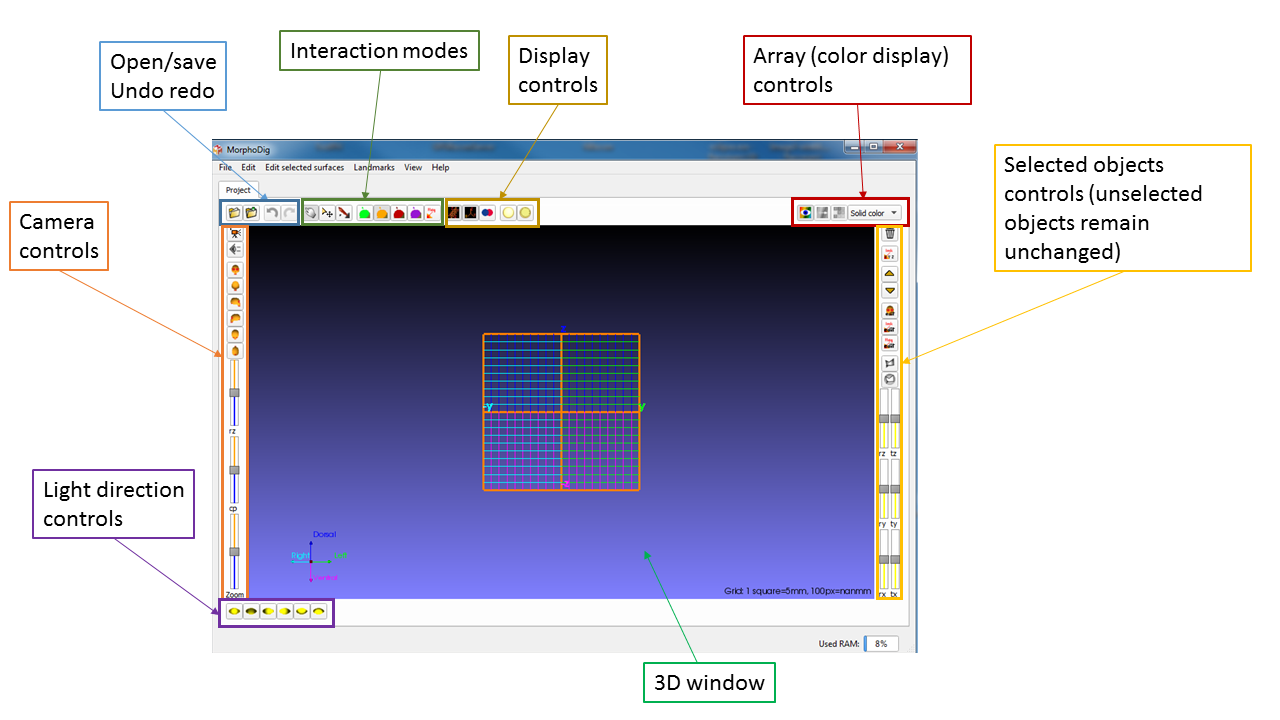
\includegraphics[scale=0.3]{images/03/morphodig_gui.png} 
	\caption{MorphoDig's GUI. Controls are organized around the main 3D rendering window.}
\label{gui}
 
\end{figure}

MorphoDig's main window is organized as shown in Fig. \ref{gui} p.\pageref{gui}. The most commonly used controls are directly accessible nearby the main 3D rendering window, and are sorted by function. 

 \section{Open and save data}


\begin{itemize}
\item There are three main ways to open data in MorphoDig. First, you can open specific files via the menu "File". You may also open data by clicking on the "open" (
\includegraphics[scale=0.03]{images/03/open_data.png}) button inside the main window (or press "CTRL +O"). You may also drag and drop files within the main 3D window.  
STL, PLY and VTK polydata surface files can be opened by MorphoDig, and many files specific to that software (files, curves, positions, color maps, tag maps, orientation-helper labels etc.).
\item In most cases, only selected objects (or some of their properties) can be saved; most "save" functionalities will not affect unselected objects. There are two main ways to save data in MorphoDig. First, you can save specific files through the menu "File". You may also save a project with the button "save project" (
\includegraphics[scale=0.03]{images/03/save_data.png})  inside the main window. Only selected objects will be considered when saving a project.
\end{itemize}





\section{Undo-Redo actions}

\begin{itemize}
\item Most actions, such as opening data, deleting data, selecting/unselecting objects, placing landmarks, modify the position of landmarks/surfaces, surface tagging etc. can be undone by clicking the "undo" button (
\includegraphics[scale=0.05]{images/03/undo.png}).
\item The same actions can be redone by clicking on the "redo" button (
\includegraphics[scale=0.05]{images/03/redo.png}).
\end{itemize}


		 \chapter{Interactions and color display. }
\minitoc  


\section{Interacting with objects}
One very important aspect of MorphoDig's design is that most interactions or modifications of opened objects can only be done when these objects are selected. 
Selected objects (3D surfaces and landmarks) are always drawn in ``grey". All currently opened objects can be selected by pressing CTRL+A. All currently opened objects can be unselected by pressing CTRL+D. Objects can also be selected/unselected using the right mouse button, depending on the currently active interaction mode (see below).



\section{Interactions modes}

See Fig. \ref{gui} p.\pageref{gui} to find the location of the "Interaction modes" controls in the main Window.
\subsection{Camera mode}
  
\includegraphics[scale=0.7]{images/04/camera_mode.png}``Camera mode" is the default interaction mode, and is active on startup. When active, left and middle mouse button drags result in camera rotation/translation, respectively. Right mouse button drag results in object selection/unselection. Pressing "ESC" switches between object mode and camera mode.
\subsection{Object mode}
   
\includegraphics[scale=0.7]{images/04/move_mode.png}When active, left and middle mouse button drags result in object rotation/translation, respectively. Right mouse button drag results in object selection/unselection. Pressing "ESC" switches between object mode and camera mode.
\subsection{Landmark mode}
  
\includegraphics[scale=0.7]{images/04/Landmarks2.png}When active, only landmarks can be selected/unselected via right mouse button drag. This mode is useful when editing/placing landmarks. Left and middle mouse button drags result in camera rotation/translation, respectively.

\section{Landmark setting modes}
Landmarks can be set on surfaces by pressing ``L" + left mouse click. 
Four series of landmarks can be set with MorphoDig: ``normal" landmarks, ``target" landmarks, ``curve node" landmarks and ``curve handle" landmarks. Additionally a fourth special landmark series (``flag" landmarks) can be used to label surface structures. 

\subsection{Normal landmark mode}	
Press ``
\includegraphics[scale=0.7]{images/04/normal_landmarks.png}" to activate this mode (this mode is active by default)

\subsection{Target landmark mode}	
Press ``
\includegraphics[scale=0.7]{images/04/target_landmarks.png}"  to activate this mode

\subsection{Curve node mode}	
Press ``
\includegraphics[scale=0.7]{images/04/curve_nodes.png}" to activate this mode 

\subsection{Curve handle mode}	
Press ``
\includegraphics[scale=0.7]{images/04/curve_handles.png}"  to activate this mode


\subsection{Flag landmark mode}	
Press ``
\includegraphics[scale=0.7]{images/04/flag_landmarks.png}" to activate this mode


 \section{Unselected surfaces color display}
See Fig. \ref{gui} p.\pageref{gui} to find the location of the "Array controls", which impact the color display of the surfaces.
 A given unselected surface can be colored: 
\begin{itemize}
\item using a uniform ``solid" color (Fig. \ref{4color_modes}-A p.\pageref{4color_modes}). Scalar display mode must be deactivated or active array combo box set to ``Solid color" (
\includegraphics[scale=0.5]{images/04/scalarcombo_solidcolor.png})
\item	according to the scalar values (= numbers) associated at the vertices (Fig. \ref{4color_modes}-B p.\pageref{4color_modes}). Array display mode button must be pressed (
\includegraphics[scale=0.7]{images/04/show_color_scale.png}), and a Scalar array must be selected (ex:
\includegraphics[scale=0.5]{images/04/scalarcombo_scalar.png}). The way scalar arrays are translated into colors can be set up using color "Lookup tables" (LUT), also referred to as color transfer functions. The "Scalar rendering options" window can be opened by clicking on "
\includegraphics[scale=0.7]{images/04/color_scale_edit.png}". 
\item according to the tag values (= integers) associated to the vertices (Fig. \ref{4color_modes}-C p.\pageref{4color_modes}). Array display mode button must be pressed (
\includegraphics[scale=0.7]{images/04/show_color_scale.png}), and a Tag array must be selected (ex:
\includegraphics[scale=0.5]{images/04/scalarcombo_tag.png}). The way Tag arrays are translated into colors can be set up using color "Lookup tables" (LUT), also referred to as color transfer functions. The "Tag options" window, in which lookup tables associated to tag arrays can be edited, can be opened by clicking on "
\includegraphics[scale=0.7]{images/04/tag_edit.png}"
\item	according to RGB values directly associated to the vertices (Fig. \ref{4color_modes}-D p.\pageref{4color_modes}). Array display mode button must be pressed (
\includegraphics[scale=0.7]{images/04/show_color_scale.png}), and a RGB array must be selected (ex:
\includegraphics[scale=0.5]{images/04/scalarcombo_rgb.png}) 
\end{itemize}

\begin{figure}
  \centering
  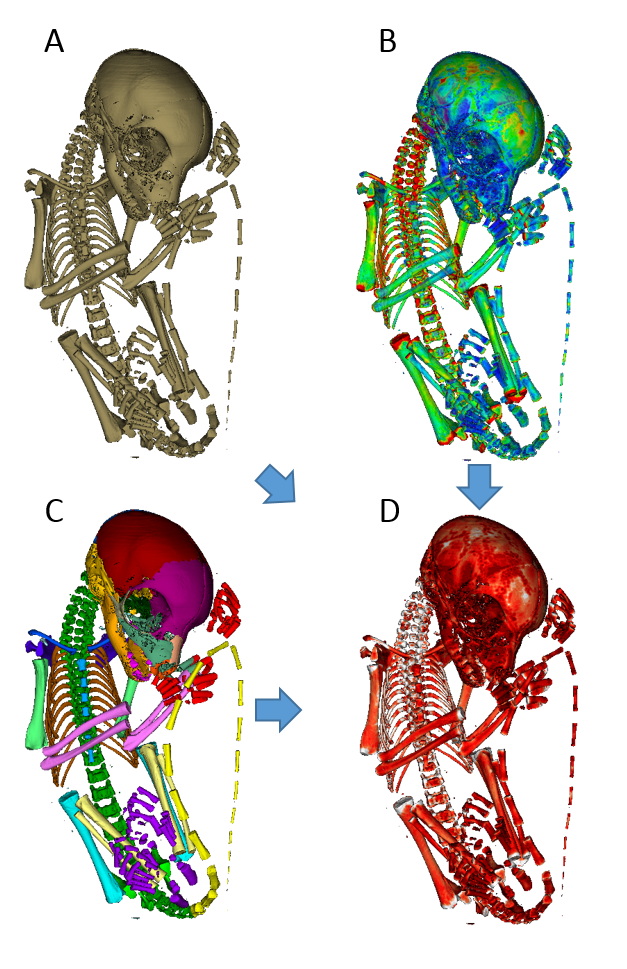
\includegraphics[scale=0.39]{images/04/4color_modes.png} 
	\caption{Color modes for a given surface. Single surface representation of the skeleton of a newborn \textit{Lemur catta}. A: "Solid color mode" mode : a uniform color is used to represent the whole surface. B: "Scalar array" representation mode. Numbers (here bone thickness) are associated to each vertex of the surface, and are rendered using a color map. C: "Tag array". Integers are associated to each vertex  (here different integer values are associated to different groups of bones), and a color map is used  to colorize the specimen. D : "RGB array" : red, green, blue and transparency information is directly associated to each vertex: no color map is used in that case. In MorphoDig, RGB arrays can be produced out of solid color information, scalar arrays and tag arrays. PLY file produced via surface scans often contain surch RGB information.}
\label{4color_modes}
 
\end{figure}
	   \chapter{Keyboard and mouse controls}
\minitoc  

 \section{Keyboard and mouse controls}
\rowcolors{2}{}{gray!25}
\begin{tabularx}{\linewidth}{ | c | X | }
 \hline			
   Ctrl+A & Selects all objects \\ \hline				
   Ctrl+D & Unselects all objects \\ \hline				
	 Ctrl+Z & Undo last action \\ \hline				
	Ctrl+Y & Redo last action \\ \hline				
   L+ left click & Creates a landmark (either ``normal", ``target", ``curve node", ``curve handle" or ``flag" landmark). \\ \hline			
L + right click & If a single landmark is selected, its position is
moved. Nothing happens if no landmark is selected
or if more than one landmark are selected \\ \hline			

Left mouse button drag 
& Camera mode : camera rotation.\newline
 Object mode : object rotation.\newline
Landmark mode : camera rotation. \\ \hline			

Ctrl + left mouse button drag 
& Camera mode : object rotation.\newline
 Object mode : camera rotation.\newline
 Landmark mode : object rotation. \\ \hline	
		
Right mouse button drag & Draws a yellow rectangle. Once right button is
released, all objects (surfaces and landmarks)
falling inside the rectangle get selected/unselected,
depending on their initial selection status \\ \hline	
		

Middle mouse button roll (roll wheel) & Zoom / unzoom \\ \hline		
	
Middle mouse button drag 
& Camera mode : camera translation\newline
 Object mode : object translation\newline
 Landmark mode : camera translation \\ \hline	
		
Ctrl + middle mouse button drag 
& Camera mode : object translation\newline
Object mode : camera translation\newline
Landmark mode : object translation \\ \hline			

« Del » & All selected objects are deleted \\ \hline			

T + left click & Picks a vertex and tags corresponding surface with active tag value (a tag array must be active, and tag mode must be activated)  \\ \hline			
 
T + right click & Picks a vertex and tags corresponding surface with active tag value (a tag array must be active, and tag mode must be activated). The only potentially affected vertices are those having initially the same color as that of the picked vertex.   \\ \hline			

 \end{tabularx}

\section{Additional controls}
Additional controls are available when using ``lasso cut" or ``lasso tag" (lasso mode should be active):\\
\begin{tabularx}{\linewidth}{ | c | X | }
\hline			
Left mouse click and drag & Draws  the lasso polygon contour\\ \hline			

Left mouse release &  all the vertices falling within the polygonal region (outside or inside the polygon) are either:\newline
- given the color corresponding the active tag (lasso tag)\newline
- inserted into a new object (lasso cut inside).\newline 
- deleted from the new object (lasso cut outside).\newline 
See lasso cut (section \ref{lasso_cut_section} p.\pageref{lasso_cut_section}) and lasso tag (section \ref{lasso_tag_section} p.\pageref{lasso_tag_section}) sections for further information.\\ \hline	
		

\end{tabularx}


		 \chapter{Main window controls}
\minitoc  


See Fig. \ref{gui} p.\pageref{gui} to have an overview of the controls described in this chapter.

%\section{Open and save data }
%\section{Undo and redo actions }


 \section{Camera controls}
Most camera related controls lay on the left part of the main window. See Fig. \ref{gui} p.\pageref{gui} to find the location of the "Camera" controls in the main Window.
\subsection{Camera rotation center}
By default, the camera rotates around the origin of the coordinate system (x=0, y=0, z=0), but by pressing ``
\includegraphics[scale=0.7]{images/06/camera/move_cam.png}"/``\includegraphics[scale=0.7]{images/06/camera/move_cam2.png}", the camera will revolve around the center of mass of all opened objects. The latter option is useful when the centre of mass of an object (or of several ones) is far from the origin of the coordinate system. The grid is drawn using different colors depending on the camera rotation centre (see Fig. \ref{grid_color} p.\pageref{grid_color}). %The camera centre can also be set at the location of one of the first 10 ``normal" landmarks (see section \ref{camera_centre_at}).

\begin{figure}
  \centering
  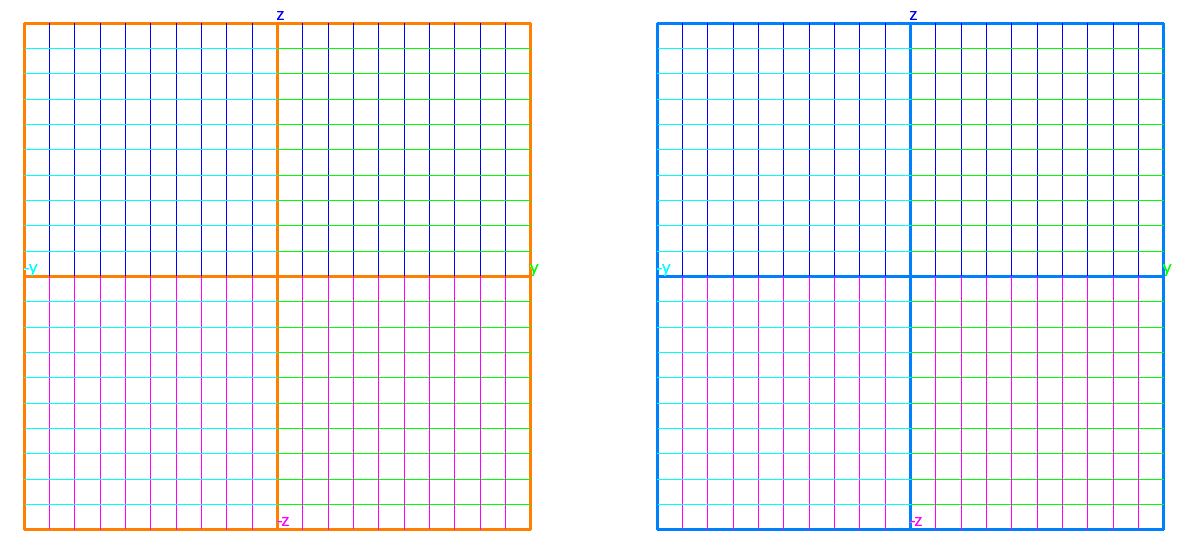
\includegraphics[scale=0.4]{images/06/camera/grids.png} 
	\caption{Grid display color. Left: when the camera revolves around the origin of the coordinate system (x=0, y=0, z=0), the grid outline is displayed in orange. Right: when the camera revolves around the center of mass of all opened objects, the grid has a blue outline.}
\label{grid_color}
 
\end{figure}

 
\subsection{Orthographic or perspective camera projection}
You can switch between orthographic and perspective projection mode by pressing the "
\includegraphics[scale=0.7]{images/06/camera/camera_ortho.png}" or "
\includegraphics[scale=0.7]{images/06/camera/camera_persp}" toggle button (see also see Fig. \ref{camera_ortho_example} p.\pageref{camera_ortho_example}).
Note that in orthographic camera projection mode 
\includegraphics[scale=0.7]{images/06/camera/camera_ortho.png}, when the grid is displayed, the relationship between pixel size on the screen and real world dimensions appears on the right bottom corner of the screen: 
\includegraphics[scale=0.7]{images/06/camera/grid_infos.png}. 

\begin{figure}
  \centering
  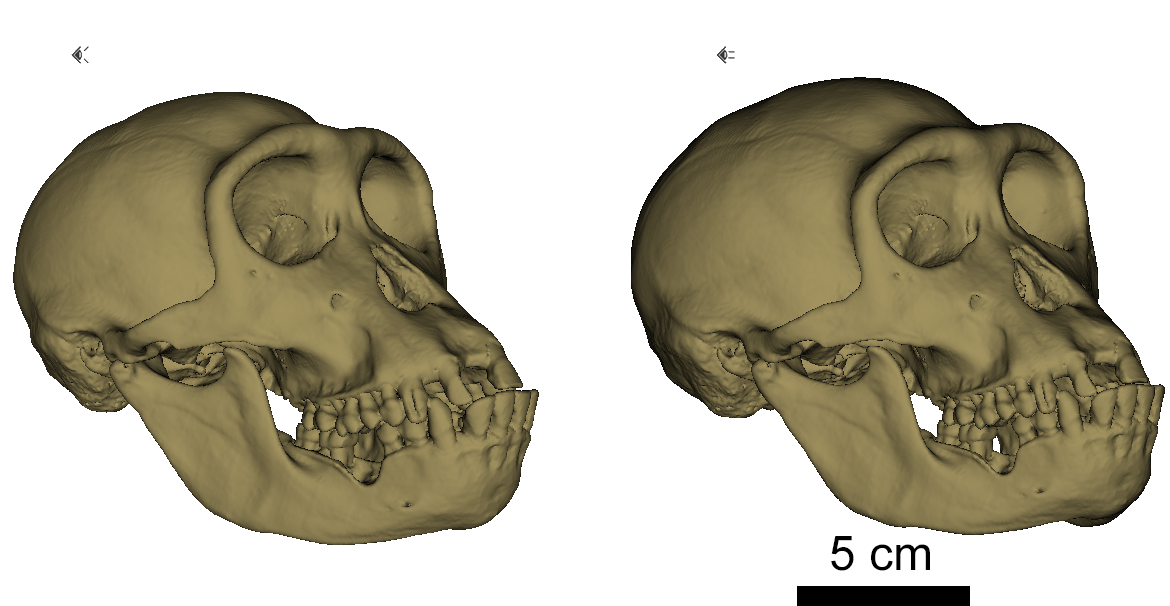
\includegraphics[scale=0.4]{images/06/camera/camera_ortho_example.png} 
	\caption{Perspective and Orthographic camera projection modes. Skull of \textit{Pan paniscus}. Left: perspective camera projection mode: closer structures appear larger than farther structures. Right: orthographic camera projection mode: a uniform relation exists between pixel size and real world dimensions, making it possible to place a scale bar. }
\label{camera_ortho_example}
 
\end{figure}


\subsection{Camera orientation}
6 camera positions are predefined :\\

\includegraphics[scale=0.7]{images/06/camera/camera_right.png} view object from right side \\

\includegraphics[scale=0.7]{images/06/camera/camera_left.png} view object from left side\\

\includegraphics[scale=0.7]{images/06/camera/camera_front.png} view object from front side (default camera position)\\

\includegraphics[scale=0.7]{images/06/camera/camera_back.png} view object from back side\\

\includegraphics[scale=0.7]{images/06/camera/camera_above.png} view object from above\\

\includegraphics[scale=0.7]{images/06/camera/camera_below.png} view object from below\\

\subsection{Screenshot}
Press "
\includegraphics[scale=0.7]{images/06/camera/screenshot.png}" to take a screenshot (.png format). Once you have defined This opens the following

\subsection{Camera rotation around ``z" viewing axis}

\begin{minipage}{0.7\textwidth}
To do so, you may use the slider lying around the center of the left panel of the main window.
\end{minipage}    
\begin{minipage}{0.25\textwidth}\centering
  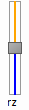
\includegraphics[scale=0.7]{images/06/camera/rz_cam.png}
 \captionof{figure}{Camera ``z" rotation slider}
 \end{minipage}    



\subsection{Clipping plane slider}

\begin{minipage}{0.7\textwidth}
In some cases, you may need to displace the viewing clipping plane. To do so, use
the slider lying centrally in the left panel of the main window. See \ref{Clipping_plane} p.\pageref{Clipping_plane} for additional clipping plane functionalities.\\

\end{minipage}    
\begin{minipage}{0.25\textwidth}\centering
  
\includegraphics[scale=0.5]{images/06/camera/cp_slider.png}
 \captionof{figure}{Camera clipping plane slider}
 \end{minipage}   




\subsection{Zoom}
There are three main ways to modify the ``zoom" in MorphoDig :


\begin{minipage}{0.7\textwidth}
\begin{itemize}
\item You may use the zoom slider laying in the lower part of the left panel of the main window.
\item	You may set manually the display scale (Edit $\rightarrow$  Edit size unit and grid spacing, then define the display scale: 100 pixels in size unit). This option is only available in orthographic projection mode 
\includegraphics[scale=0.7]{images/06/camera/camera_ortho.png}.
\item	You may use the middle click mouse roll button (roll the wheel).
\end{itemize}
\end{minipage}    
\begin{minipage}{0.25\textwidth}\centering
  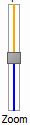
\includegraphics[scale=0.5]{images/06/camera/zoom_slider.png}
 \captionof{figure}{Zoom slider}


 \end{minipage}    


\section{Display controls}
The display controls mentioned in this section are situated on the top part of the main window (see Fig. \ref{gui} p.\pageref{gui}).


\subsection{Grid}
Press 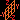
\includegraphics[scale=0.7]{images/06/display/grid.png} to show / hide the grid. Default grid size is 1 cm / square. Grid size can be edited manually
(viewing opt. $\rightarrow$ Grid size).
Switching between the 6 camera predefined positions defined above (
\includegraphics[scale=0.7]{images/06/camera/camera_right.png}, 

\includegraphics[scale=0.7]{images/06/camera/camera_left.png}, 

\includegraphics[scale=0.7]{images/06/camera/camera_front.png}, 

\includegraphics[scale=0.7]{images/06/camera/camera_back.png}, 

\includegraphics[scale=0.7]{images/06/camera/camera_above.png} and 
\includegraphics[scale=0.7]{images/06/camera/camera_below.png})
will affect the plane in which the grid is drawn.




\subsection{Coordinate system orientation helper}
\begin{minipage}{0.7\textwidth}
Press \includegraphics[scale=0.7]{images/06/display/orientation_helper.png} to show / hide the coordinate system orientation helper lying on the bottom left corner of the main 3D window. By default, the labels are defined
the following way:\\
+z axis : dorsal side\\
-z axis : ventral side\\
+y axis : left side\\
-y axis : right side\\
+x axis : anterior side\\
-x axis : posterior side.\\
You may edit these labels depending on your preferences (for instance,
depending on the structure you are working with, you may need to set ``+y" to ``labial", and ``-y" to
``lateral"). To edit orientation labels, click on ``Edit $\rightarrow$ Edit orientation labels."
\end{minipage}    
\begin{minipage}{0.3\textwidth}\centering
 \includegraphics[scale=0.7]{images/06/camera/orientation_helper_view.png}
 \captionof{figure}{Orientation helper}
 \end{minipage}   


\subsection{Anaglyph}
Press \includegraphics[scale=0.7]{images/06/display/anaglyph.png} to activate/deactivate anaglyph 3D rendering.
See Fig. \ref{anaglyph_example} p.\pageref{anaglyph_example}. You then need to wear "Red/Blue" \includegraphics[scale=0.7]{images/06/display/anaglyph_glasses.png} glasses to visualize objects in 3D.

\begin{figure}
  \centering
  \includegraphics[scale=0.34]{images/06/display/anaglyph_example.png} 
	\caption{Anaglyph display mode. Left: normal display mode. Right: anaglyph display mode. Cranium of the holotype specimen of \textit{Pan paniscus}.}
\label{anaglyph_example}
 
\end{figure}



%You can also modify the clipping plane manually by editing the ``Tz" control in the camera options window (viewing opt. $\rightarrow$ Camera $\rightarrow$ Camera options).

\subsection{Clipping plane} \label{Clipping_plane}

The button \includegraphics[scale=0.7]{images/06/display/cpon.png} or \includegraphics[scale=0.5]{images/06/display/cpoff.png}  permits to adjust / readjust the position of the clipping plane at predefined positions (see for instance Fig. \ref{cp_example} p.\pageref{cp_example}):
\begin{itemize}
\item  \includegraphics[scale=0.7]{images/06/display/cpon.png}: the clipping plane is placed at z = 0 (all objects having a z coordinate along
z viewing axis smaller than 0 are hidden).
\item	\includegraphics[scale=0.7]{images/06/display/cpoff.png} : the clipping plane is replaced at its original value : z= - camera.far / 2. This value permits to
view objects having positive and negative coordinates along z viewing axis.

\end{itemize}
\begin{figure}
  \centering
  \includegraphics[scale=0.4]{images/06/display/cp_example.png} 
	\caption{Clipping plane display mode. Cranium of the type specimen of \textit{Pan paniscus}. Left: normal display mode. Right: clipping plane display mode "on" : permits to visualize inner structures. }
\label{cp_example}
 
\end{figure}



\subsection{Backface culling} \label{Backface_culling}

Hiding backfaces of a surface is useful in some cases to visualize inner structures of a biological object (see for instance Fig. \ref{backface_example} p.\pageref{backface_example}). The button \includegraphics[scale=0.7]{images/06/display/backface_on.png} / \includegraphics[scale=0.7]{images/06/display/backface_off.png}  permits to visualize/hide backfaces :
\begin{itemize}
\item  \includegraphics[scale=0.7]{images/06/display/backface_on.png}: both sides of a given surface object are rendered.
\item	\includegraphics[scale=0.7]{images/06/display/backface_off.png} : backfaces are hidden (only frontfaces are visible).

\end{itemize}


\begin{figure}
  \centering
  \includegraphics[scale=0.3]{images/06/display/backface_example.png} 
	\caption{Backface culling display mode. Petrosal bone of \textit{Eulemur mongoz}. Left: normal display mode: both frontfaces (lighter) and backfaces (darker) are displayed. Right: backface culling mode activated: only frontfaces are displayed, making it easier to visualize the bony labyrinth. }
\label{backface_example}
 
\end{figure}



\subsection{Surface 3D representation controls}


4 different options exist to draw 3D surfaces :\\
\includegraphics[scale=0.7]{images/06/display/point_normals.png} : point normals display mode (Gouraud shading), see Fig. \ref{4display_modes}-A.\\
\includegraphics[scale=0.7]{images/06/display/cell_normals.png} : triangle normals display mode, see Fig. \ref{4display_modes}-B. \\
\includegraphics[scale=0.7]{images/06/display/wireframe.png} : wireframe representation  display mode, see Fig. \ref{4display_modes}-C.\\
\includegraphics[scale=0.7]{images/06/display/points.png} point cloud display mode, see Fig. \ref{4display_modes}-D\\

\begin{figure}
  \centering
  \includegraphics[scale=0.4]{images/06/display/4display_modes.png} 
	\caption{Display modes available for a given surface. Single surface representation of the left bony labyrinth of a  \textit{Lepilemur dorsalis}. A: "Point normales" mode (Gouraud shading). B: "Triangle normales" mode. C: "Wireframe" mode. D: "Point cloud" mode.}
\label{4display_modes}
 
\end{figure}


\section{Light direction controls}
See Fig. \ref{gui} p.\pageref{gui} to see where the "light controls" are situated within MorphoDig's main window.


6 lightning orientations are predefined :\\
\includegraphics[scale=0.7]{images/06/light/light_right.png}light from right viewing side\\
\includegraphics[scale=0.7]{images/06/light/light_left.png}light from left viewing side\\
\includegraphics[scale=0.7]{images/06/light/light_front.png}light from front viewing side\\
\includegraphics[scale=0.7]{images/06/light/light_back.png}light from back viewing side\\
\includegraphics[scale=0.7]{images/06/light/light_above.png}light from above\\
\includegraphics[scale=0.7]{images/06/light/light_below.png}light from below\\




  \section{Object controls}
See Fig. \ref{gui} p.\pageref{gui}to see where the "object controls" are situated within MorphoDig's main window. Remind that only selected objects are affected by these controls.

\subsection{Delete selected objects}
Clicking on "\includegraphics[scale=0.7]{images/06/objects/delete2.png}" deletes all selected objects. This action can be undone/redone.

\subsection{Create landmark at X,Y,Z}
Clicking on "\includegraphics[scale=0.7]{images/06/objects/landmark_xyz.png}" opens the "Create landmark" window  (Fig. \ref{create_landmark} p.\pageref{create_landmark}), in which a new landmark can be created a specified coordinates. This action can be undone/redone..

\begin{figure}
  \centering
  \includegraphics[scale=0.55]{images/06/objects/create_landmark.png} 
	\caption{Create landmark at a given X,Y,Z coordinate.}
\label{create_landmark}
 
\end{figure}
\subsection{Decrease / Increase landmark number}
Clicking on \includegraphics[scale=0.7]{images/06/objects/move_up.png} will increase (= move down in list, if possible) the landmark number of all selected landmarks. Clicking on \includegraphics[scale=0.7]{images/06/objects/move_down.png} will decrease (=move up in list, if possible) the landmark number of all selected landmarks. These buttons make it possible to reorder landmarks.
\subsection{Edit first selected surface}

Clicking on "\includegraphics[scale=0.7]{images/06/objects/actor_edit.png}" opens the "Edit first selected surface" window (Fig. \ref{actor_edit} p.\pageref{actor_edit}), in which several properties of a given surface object can be edited.
\\
- Object name : modifies the name of the object.\\
- Next object \includegraphics[scale=0.7]{images/06/objects/s_right.png} and preceding object \includegraphics[scale=0.7]{images/06/objects/s_left.png}: saves currently  settings and fetches next/preceding surface.\\
- Object solid color : modifies the "solid color" property of this object.\\
- Object translucency : modifies the translucency this object.
- Object matrix : current position/rotation matrix of the object.\\
- Reinit matrix: set current matrix to identity.\\
- Apply matrix to all selected surfaces : set position/rotation matrix to all other selected surfaces.\\
- Existing arrays : list of all scalar/RGB color/tags arrays associated to the vertices of the surfaces.\\
- Edit array name : modifies the name of currently selected array\\
- Duplicate array : duplicates currently selected array\\
- Delete array : deletes currently selected array\\
- Ok : save settings and closes window



\begin{figure}
  \centering
  \includegraphics[scale=0.55]{images/06/objects/edit_surface.png} 
	\caption{Edit first selected surface window.}
\label{actor_edit}
 
\end{figure}



\subsection{Edit first selected landmark}
Clicking on "\includegraphics[scale=0.7]{images/06/objects/landmark_edit.png}" opens the "Edit first selected landmark" window (Fig. \ref{landmark_edit} p.\pageref{landmark_edit}), in which landmark coordinates of landmarks can be manually edited. The center of rotation of the camera can be set to the x,y,z coordinates of a given landmark by pressing on "\includegraphics[scale=0.7]{images/06/objects/move_cam3.png}".




\begin{figure}
  \centering
  \includegraphics[scale=0.55]{images/06/objects/edit_landmark.png} 
	\caption{Edit first selected landmark window.}
\label{landmark_edit}
 
\end{figure}

\subsection{Edit first selected flag}
Clicking on "\includegraphics[scale=0.7]{images/06/objects/flag_edit.png}" opens the "Edit first selected flag" window (Fig. \ref{flag_edit} p.\pageref{flag_edit}), in which several properties of a given flag can be manually edited.

- Flag name : modifies the label of this flag.\\
- X, Y, Z: 3D coordinates of the flag.\\
- Next flag \includegraphics[scale=0.7]{images/06/objects/s_right.png} and preceding flag \includegraphics[scale=0.7]{images/06/objects/s_left.png}: saves currently  settings and fetches next/preceding flag\\
- Flag color : modifies the "color" of the currently selected flag.\\
- Flag rendering size : modifies the length of the flag.\\
The center of rotation of the camera can be set to the x,y,z coordinates of a given flag by pressing on "\includegraphics[scale=0.7]{images/06/objects/move_cam3.png}".


\begin{figure}
  \centering
  \includegraphics[scale=0.55]{images/06/objects/edit_flag.png} 
	\caption{Edit first selected flag window.}
\label{flag_edit}
 
\end{figure}

\subsection{Lasso cut selected surfaces} \label{lasso_cut_section}

You may cut through an input selected surface using this option (see Fig. \ref{lasso_cut} p.\pageref{lasso_cut}). Once "\includegraphics[scale=0.7]{images/06/objects/lasso_keepinside.png}" (lasso cut keep inside) or "\includegraphics[scale=0.7]{images/06/objects/lasso_keepoutside.png}" (lasso cut keep outside) button has been pressed, the mouse cursor changes and you can start drawing the lasso section by dragging the mouse while the left button is pressed. When the left button is released, the lasso cut operation starts: a new object is created, which contains all the parts of the selected object laying inside or outside the drawn polygon, respectively.\\

\begin{figure}
  \centering
  \includegraphics[scale=0.6]{images/06/objects/lasso_cut.png} 
	\caption{A: "Lasso keep outside" button is pressed, then a polygon is drawn over the selected object (grey) by maintaining left mouse button pressed and dragging the mouse. B: Left mouse button has been released: a new surface object is  created. C: "Delete" has been pressed : only the newly created  object remains. C: "Lasso keep inside" is pressed, then a polygon is drawn over the selected object (grey) by maintaining left mouse button pressed and dragging the mouse. E: Left mouse button has been released : a new surface object is  created. F: "Delete" has been pressed : only the newly created  object remains. }
\label{lasso_cut}
 
\end{figure}

\subsection{Rubber band cut selected surfaces} \label{rubber_band_cut_section}

You may cut through an input selected surface using this option (see Fig. \ref{rubber_band_cut} p.\pageref{rubber_band_cut}). Once "\includegraphics[scale=0.7]{images/06/objects/rubber_mode_keepinside.png}" (rubber band cut, keep inside) or "\includegraphics[scale=0.7]{images/06/objects/rubber_mode_keepoutside.png}" (rubber band cut, keep outside) button has been pressed, the mouse cursor changes and you can start drawing a rectangular section by dragging the mouse while the left button is pressed. When the left button is released, the rubber band cut operation starts: a new object is created, which contains all the parts of the selected object laying inside or outside the drawn rectangle, respectively.\\

\begin{figure}
  \centering
  \includegraphics[scale=0.6]{images/06/objects/rubber_band_cut.png} 
	\caption{A: "Rubber band cut keep inside" button is pressed, then a rectangle is drawn over the selected object (grey) by maintaining left mouse button pressed and dragging the mouse. B: Left mouse button has been released: a new surface object is  created. C: "Delete" has been pressed : only the newly created  object remains. C: "Rubber band cut keep outside" is pressed, then a rectangle is drawn over the selected object (grey) by maintaining left mouse button pressed and dragging the mouse. E: Left mouse button has been released : a new surface object is  created. F: "Delete" has been pressed : only the newly created  object remains. }
\label{rubber_band_cut}
 
\end{figure}

\subsection{object rotation and translation sliders}
	As seen earlier, selected objects can be translated and rotated using the mouse left and middle buttons
(in landmark and camera selection modes, you also need to maintain ``CTRL" button pressed
while dragging the mouse to achieve rotation and translation of selected objects). Alternatively, you
may also use the following controls to accomplish rotation and translation of selected objects. Rotation
is performed around the global center of mass of all currently selected objects.

\subsubsection{Rotation around and translation along ``Z" viewing axis }

These controls are extremely useful, as there is no way to achieve rotation round « z » viewing axis or translation along ``z" viewing axis using the
mouse. \\ To do so, use the tz and rz sliders (see Fig. \ref{move_z} p.\pageref{move_z}).


\begin{figure}
  \centering
  \includegraphics[scale=0.45]{images/06/objects/move_objects_z.png} 
	\caption{A: object and tz slider are in initial position. B: tz slider is moved down: the selected object moves forward. C: tz slider is moved up. The selected object moves backward. D: object and rz slider are in initial position. E: rz slider is moved down: the selected object rotates around the "roll" axis counter-clockwise. F: rz slider is moved up. The selected object rotates around the "roll" axis clockwise.}
\label{move_z}
 
\end{figure}



\subsubsection{Rotation/translation around/along ``Y" viewing axis}

To do so, use the ty and ry sliders (see Fig. \ref{move_y} p.\pageref{move_y}).

\begin{figure}
  \centering
  \includegraphics[scale=0.45]{images/06/objects/move_objects_y.png} 
	\caption{A: object and ty slider are in initial position. B: ty slider is moved down: the selected object moves downward. C: ty slider is moved up. The selected object moves upward. D: object and ry slider are in initial position. E: ry slider is moved down: the selected object rotates around the "yaw" axis clockwise. F: ry slider is moved up. The selected object rotates around the "yaw" axis counter-clockwise.}
\label{move_y}
 
\end{figure}



\subsubsection{Rotation/translation around/along ``X" viewing axis}

To do so, use the ty and ry sliders (see Fig. \ref{move_x} p.\pageref{move_x}).

\begin{figure}
  \centering
  \includegraphics[scale=0.45]{images/06/objects/move_objects_x.png} 
	\caption{A: object and tx slider are in initial position. B: tx slider is moved down: the selected object moves leftward. C: tx slider is moved up. The selected object moves rightward. D: object and rx slider are in initial position. E: rx slider is moved down: the selected object rotates around the "pitch" axis clockwise. F: rx slider is moved up. The selected object rotates around the "pitch" axis counter-clockwise.}
\label{move_x}
 
\end{figure}
		 \chapter{Menu File}
\minitoc  


\section{Project}
When working with multiple surface objects, loading surfaces and associated positions one by one becomes fastidious. Besides, after having digitized landmarks, flags, after having set tag names and colors, or after having defined orientation labels, you may wish to open or save this information along with surface files. You may open and save series of surface files and associated position matrices, landmarks, flags, tag colors and labels and orientation labels using this menu. ``Project" files (.ntw) files are organized the following way (see Fig. \ref{project_file}):\\
- Optional: name of orientation label file (.ori)\\
- Optional: name of tag file (.tag)\\
- Optional: name of flag file (.flg)\\
- Optional: name of landmak file (.lmk, .ver, .stv or .cur)\\
- Name of surface 1 file\\
- Name of position 1 file associated to surface 1\\
- Surface 1 RGB color and transparency\\
- Name of surface 2 file\\
- Name of position 2 file associated to surface 2\\
- Surface 2 RGB color and transparency (etc...)\\
 
Surface files can be of the following types : .stl, .vtk and .ply\\
``.ntw" files can be constructed manually, providing that the referred surface and position files exist.



\begin{figure}
  \centering  
 \includegraphics[scale=0.5]{images/07/project/ntw.png}
 \captionof{figure}{Example of project .ntw file containing references to orientation labels, tags labels and colors, flags and landmarks files.}
\label{project_file}
\end{figure}

\subsection{Open project}
Loads a .ntw file

\subsection{Save project}
\begin{figure}
  \centering  
 \includegraphics[scale=0.5]{images/07/project/save_ntw.png}
 \captionof{figure}{Save project window.}
\label{save_project_file}
\end{figure}
Behavior: only selected elements (surface objects, landmarks, flags...) are saved within projects. If at least one opened element has been selected, the Save project window (\ref{save_project_file}) opens and asks whether :  
\begin{itemize}
\item orientation labels should be saved along with the project (by default, orientation labels are not saved, as orientation labels are quite rarely set by users). 
\item tag legends and colors (tag maps) should by saved. By default, .tag file are not saved along with the project, as tag setting is not a common task. 
\item save surfaces as. VTK polydata or PLY. We advise you to save your surfaces as VTK polydata. In the contrary cases scalar,  tag arrays and all RGB arrays having a name different from "RGB" will be lost.
\item save position inside .POS file, or apply the position to surfaces. We advise you to save position inside .POS file (otherwise, the initial orientations of your surfaces will be lost). 
\end{itemize}
Each surface file will be given the name of the original file. Each position file will be given a name which starts with the name of the associated surface and ends with the name of the project (1 exception: when the project contains only one surface and  the project's name is the same as that of the surface. In that case, .pos file names are not postfixed with the name of the project). In the .ntw file example shown in Fig. \ref{project_file}, the surface files are 
\begin{itemize}
\item ``Hippopotamus\_amphibius\_braincase.vtk" 
\item ``Hippopotamus\_amphibius\_bulla.vtk" 
\item ``Hippopotamus\_amphibius\_petrosal.vtk" 
\item ``Hippopotamus\_amphibius\_sinus.vtk" 
\end{itemize}
\noindent and the project name is ``exploded.ntw". The advantage of naming position files that way is you may construct different .ntw files with different associated surface files using a same set of surfaces. Requirement : all selected surfaces saved via this option
need to have distinct names. Note : When working with ``project" files, if several surface objects have the same name, you may need at
some point to rename some of the object surfaces in order to make sure that all surface objects have a distinct name. To do so, select one surface, click on \includegraphics[scale=0.7]{images/06/objects/actor_edit.png}: the ``Edit first selected surface" window appears (See Fig. \ref{actor_edit} in preceding chapter).




\section{Surface}
\subsection{Open surface}
STL, PLY and VTK polydata surfaces can be open via this menu. MorphoDig does not manage textures associated with surface files. When opening a PLY file containing RGB colors (for instance a file painted manually or automatically with ``MeshLab", or some laser scanner surface files) or a VTK file containing RGB arrays, these colors are placed inside a (or several) "RGB" array(s). 
%MorphoDig will reinitialize the ``RGB" scalars whenever you change the object's color or whenever you activate tag display mode or scalar display mode : if these colors are important to you, you may convert them to TAG values in the menu Tags$\rightarrow$Convert RGB colors to tags before changing the object color or display mode/before changing tags or any color scale activated.

\subsection{Save surface}
Selected surfaces can be saved into files. If no surface is selected, the following message appears:\\
\includegraphics[scale=0.5]{images/07/surface/no_surface_selected.png}\\
If at least 2 surfaces are selected, the following message shows up:\\
\includegraphics[scale=0.5]{images/07/surface/at_least_2_surfaces_selected.png}

\subsubsection{Save selected surfaces in one single .PLY file}

\begin{minipage}{0.5\textwidth}
Options:
\begin{itemize}
\item File type: you can save .ply data in binary (little or big endian)
or ASCII formats.
\item Position : you can keep object original coordinate system or
save the surface in its current position.
\item Normals : you can chose whether you wish to save normals.
\item Colors : RGB information associated to each vertex can be saved. You may decide either to keep current RGB color array (if that array exists). Alternatively, you may decide not to save the current RGB color array (if it exists). Finally, you may prefer to save/replace the current RGB color array as the current display color.
\end{itemize}

\end{minipage}    
\begin{minipage}{0.5\textwidth}\centering
  \includegraphics[scale=0.45]{images/07/surface/save_ply.png}
 \captionof{figure}{PLY save options window}
 \end{minipage} 

Note that a "RGB" array (object rendering color, depending on which rendering mode you
are using), depending on the chosen options, can be saved inside the .ply file. This means that Tag / Scalar / Object solid color can be exported and viewed in other software such as MeshLab.


\subsubsection{Save selected surfaces in one single .VTK PolyData (.VTK or .VTP) file}
\begin{minipage}{0.5\textwidth}
VTK polydata surface file format is by far not as widespread as STL or PLY
formats. However, it is extremely useful as it allows to store several
scalar, tag and RGB arrays.
Options:
\begin{itemize}
\item File type: you can save .VTK data in binary (little endian) or
ASCII formats.
\item Position : you can keep object original coordinate system
or save the surface in its current position.
\item Arrays: you decided which arrays (scalars, tags, RGB colors) should be saved inside the VTK polydata file.
\end{itemize}
\end{minipage}    
\begin{minipage}{0.5\textwidth}\centering
  \includegraphics[scale=0.5]{images/07/surface/save_vtk.png}
 \captionof{figure}{VTK save options window}
 \end{minipage} 
\noindent


\subsubsection{Save selected surfaces in one single .STL file}

\begin{minipage}{0.5\textwidth}
Options:
\begin{itemize}
\item File type: you can save .stl data in binary (little endian) or
ASCII formats.

\item Position : you can keep object original coordinate system or save the surface in its current position
\end{itemize}

\end{minipage}    
\begin{minipage}{0.5\textwidth}\centering
  \includegraphics[scale=0.5]{images/07/surface/save_stl.png}
 \captionof{figure}{STL save options window}
 \end{minipage} 




\section{Position}
In MorphoDig, surface position consists in two
4*4 square matrices: the first matrix is currently not read nor used anymore by MorphoDig, but is kept for compatibility issues with older versions of MorphoDig and of ISE-MeshTools (MorphoDig is a major redesign of an older software, ISE-MeshTools). This first matrix will disappear in a near future.  The second matrix is the one that matters: the position matrix. It contains the rotation and translation information of 3D objects (3D surfaces and landmarks). These 2 matrices can be opened and saved in ``.pos" format (see Fig. \ref{position_file}).


\begin{figure}
  \centering
  \includegraphics[scale=0.5]{images/07/position/position_file.png}
 \caption{Example of .pos position file. The first 4 lines correspond
to the aspect matrix, and the 4 last lines to the position matrix.}
\label{position_file}
\end{figure}
 



\subsection{Open position for selected surfaces}
If no surface is selected, the following message
appears:\\
\includegraphics[scale=0.5]{images/07/position/no_surface_selected.png}
\\
If at least 2 surfaces objects are selected, the same position will be given to them.

\subsection{Open transposed position for selected surfaces}
This option may be useful in the following case:
\begin{itemize}
\item Let us suppose that you did modify the position of a given surface and saved its position.
\item Then you have saved the surface in its current modified position (= the original position of the
surface is lost).
\end{itemize}

It may happen that you need to open the surface in its original position. To do so, you may apply this option (apply transposed position matrix to the modified surface).

\subsection{Open position for selected landmarks/flags}
If no landmark/flag is selected, the following message
appears:\\
\includegraphics[scale=0.5]{images/07/position/no_landmark_selected.png}
\\
This options may be useful when you have digitized landmarks/flags on a given surface in its original position and orientation. Let us suppose that in a second step, you need to modify the position/orientation of that surface object and that you save it in a .POS file. You may then apply this .POS file to your set of landmarks/flags.

\subsection{Open transposed position for selected landmarks/flags}
If you have digitized landmarks/flags on a surface with a modified position (let us assume that the position of this surface is saved within a .POS file), by using this option, you can replace this landmarks/flags dataset on the surface in its original orientation. 


\subsection{Save position for selected surfaces}
Surface aspect and position matrices can be saved in ``.pos" format. If no surface is selected, the
following message appears:\\
\includegraphics[scale=0.5]{images/07/position/no_surface_selected.png}
\\
If at least 2 surfaces selected, the following message shows up:\\
\includegraphics[scale=0.5]{images/07/position/at_least_2_surfaces_selected.png}

\subsection{Edit manually position matrix}
Clicking on "\includegraphics[scale=0.7]{images/06/objects/actor_edit.png}" opens the "Edit first selected surface" window (Fig. \ref{actor_edit}), in which the position matrix of a given actor can be modified.



\section{Landmarks}
Landmarks can be set on surfaces by pressing ``L" + left mouse click.\\

Two series of conventional landmarks can be set : ``normal" and ``target" landmarks. In the ``normal" landmark mode (button \includegraphics[scale=0.7]{images/04/normal_landmarks.png} active), pressing ``L" + left mouse click results in the creation a ``normal" landmark (a light green one). In the ``target" landmark mode (button \includegraphics[scale=0.7]{images/04/target_landmarks.png} active),
pressing ``L" + left mouse click will create a ``target" landmark (a yellow transparent one).

 ``Normal" and ``target" landmarks can be loaded and saved.\\
Selected landmarks can be reordered using the following buttons. Pressing ``\includegraphics[scale=0.7]{images/06/objects/move_up.png}"
will (try to) increase the number of all selected landmarks, while pressing ````\includegraphics[scale=0.7]{images/06/objects/move_down.png}""
will (try to) decrease their number, respectively.\\\\
MorphoDig can manage three types of landmark files: ``.LMK", ``.VER" and ``.STV" files.
\begin{itemize}
\item 
 .LMK files contain a series of lines, each line
being constructed the following way (see Fig. \ref{LMK_file}): landmark
name (without space or tab character),
landmark coordinates. Note that each landmark name does not need to be of the form ``landmark"+landmark number. Meanwhile, the name should not hold space or tab
characters.
\item .VER files contain a series
of lines, each line being
constructed the following
way (see Fig. \ref{VER_file}): landmark name (without space or tab character), landmark coordinates, landmark orientation.
\item STV files may contain one or two series of line. The first line contains two integers, the first being the type of landmark (0 for ``normal" or 1 for ``target"), the second being the number of lines of landmarks of this type which are expected to follow, constructed the following way: landmark name (without space or tab character), landmark coordinates, landmark orientation. An example of .STV file containing both ``normal" and ``target" landmarks is given in Fig. \ref{STV_file}. Note that the number of ``normal" and ``target" landmarks saved within a .STV file can differ.
\end{itemize}
\begin{figure}
  \centering
  \includegraphics[scale=0.5]{images/07/landmarks/LMK_file.png}
 \caption{Example of .LMK file}
\label{LMK_file}
\end{figure}

\begin{figure}
  \centering
  \includegraphics[scale=0.5]{images/07/landmarks/VER_file.png}
 \caption{Example of .VER file}
\label{VER_file}
\end{figure}
\begin{figure}
  \centering
  \includegraphics[scale=0.5]{images/07/landmarks/STV_file.png}
 \caption{Example of .STV file. We advise you to use this file format.}
\label{STV_file}
\end{figure}

\subsection{Open MorphoDig Landmark/Curve File (STV)}
STV file contain lists of "normal", "target" landmarks (but may also contain lists of "curve node" and "curve handle" landmarks).
\subsection{Open Landmarks}
Landmarks (.VER or .LMK) opened using this option will be put in the ``normal" landmark list (light green landmarks)
\subsection{Open Target Landmarks}
Landmarks opened using this option will be put in the ``target" landmark list (yellow transparent landmarks)
\subsection{Save MorphoDig Landmark/Curve File (STV)}
You may decide whether you wish to save all (normal, target, curve node, curve handle) landmarks or only selected ones (see Fig. \ref{save_stv}).
\begin{figure}
  \centering
  \includegraphics[scale=0.5]{images/07/landmarks/save_stv.png}
 \caption{Save STV window.}
\label{save_stv}
\end{figure}

\subsection{Save Landmarks}
You may decide whether you wish to save only selected ``normal" landmarks or all selected and
unselected ``normal" landmarks (the yellow transparent ones) in .VER or .LMK format (see Fig. \ref{save_ver_lmk}).
\begin{figure}
  \centering
  \includegraphics[scale=0.5]{images/07/landmarks/save_ver_lmk.png}
 \caption{Save Landmark Window. Used to save either "Normal", "Target" landmarks (but not both at the same time). This windows is also used to save curve nodes or curve handles in .LMK and .VER format (but also not both at the same time). }
\label{save_ver_lmk}
\end{figure}.
The ``Landmarks" chapter (chapter \ref{landmark_chapter}) and the tutorial ``working with landmarks" contain further information regarding landmark digitization with MorphoDig.


\subsection{Save Target Landmarks}
You may decide whether you wish to save only selected ``target" landmarks or all selected and
unselected ``target" landmarks (the yellow transparent ones) in .VER or .LMK format (see Fig. \ref{save_ver_lmk}).
The ``Landmarks" chapter (chapter \ref{landmark_chapter}) and the tutorial ``working with landmarks" contain further information regarding landmark digitization with MorphoDig


\section{Curves}\label{file_curve_section}

3D Curves (series of 3D cubic Bezier curves) are constructed in MorphoDig using 2 series of landmarks : a series of N ``curve node" landmarks, and a series of N ``curve handle".  Curve nodes and handles can be set on surfaces by pressing ``L" + left mouse click. In the ``curve nodes" landmark mode (button \includegraphics[scale=0.7]{images/04/curve_nodes.png} active), pressing ``L" + left mouse click results in the creation a ``curve node" landmark (a dark green for a curve starting node, and then light red ones). In the ``curve handles" landmark mode (button \includegraphics[scale=0.7]{images/04/curve_handles.png} active), pressing ``L" + left mouse click will create a ``target" landmark (a violet transparent one).

Selected curve nodes/handles can be reordered using the following buttons. Pressing ``\includegraphics[scale=0.7]{images/06/objects/move_up.png}"
will (try to) increase the number of all selected curve nodes/handles, while pressing ````\includegraphics[scale=0.7]{images/06/objects/move_down.png}""
will (try to) decrease curve nodes/handles number, respectively.\\


3D Bezier curves passing through all curve nodes are draw green when no curve node/handle belonging to
the curve segment is selected. Curves are drawn red when at least one curve node/handle involved in the
curve segment is selected. Two different cases are considered:
\begin{itemize}

\item Case 1: the numbers of ``curve node" and ``curve handle" landmarks differ. In that case, a curve is a series of lines passing through ``curve node" landmarks.
\item Case 2: the numbers of ``curve node" and ``curve handle" landmarks are equal. In that case, a curve is a
series of cubic Bezier curves passing through ``normal" landmarks. For a given set of 2 ``curve node"
consecutive landmarks (Ln and Ln+1) and their associated ``curve handles" (Hn and Hn+1), a mirror
image of Hn+1 relative to Ln+1 (H'n+1) is constructed. The Bezier curve involving Ln, Ln+1, Hn and
Hn+1 starts from Ln, going toward Hn, and arrives at Ln+1 coming from the direction of H'n+1.

\end{itemize}


The explicit form of the curve is :
\begin{equation}
B(t) = (1-t)^{3}Ln + 3(1-t)^{3}tHn + 3(1-t)t^{2}H'n+1 +t^{3}Ln+1, t \in[0,1]
\end{equation}
\\
In order to be able to digitize several curves using a given set of curve node and curve handle landmarks,
``curve node" landmarks curves can be given 4 flags (see section \ref{landmarks_curves_section} ``Landmarks $\rightarrow$ selected curve node and handle landmarks" for further details):\\
Flag ``0" : node is within a given curve segment (drawn ``red").\\
Flag ``1" : node is the starting point of a curve segment (drawn dark ``green").\\
Flag ``2" : node is placed inside the curve, and is a curve ``milestone" (drawn blue) .\\
Flag ``3" : node is placed inside the curve, and should be connected to the preceding curve
segment starting point. When curve node "N" is flagged that way, curve node "N+1" will be set automatically as a curve segment starting point.\\
Flag ``2" is used to decompose a given curve segment into curve sub-segments. By default, a curve comprises 1 segment.\\
Flag ``3" is used to close a curve (by default, curves are open).\\
3D curves are loaded and saved into either .STV (more generic) or .CUR (more specific) files. CUR files which contain a series of lines, each line being
constructed the following way: name (without space or tab character), curve ``node" landmark
coordinates, curve ``handle" coordinates, flag.
In the example shown below, 4 curves are defined :\\
- an open curve starting from curve node 1 and ending at landmark 7\\
- a closed curve involving landmarks 8 to 12\\
- an open curve involving landmarks 13 to 20\\
- a closed curve involving landmarks 21 to 26\\
These four curves contain only one sub-segment (no curve milestone was set within those 4 curves).
Note that each name does not need to be of the form ``CurvePart"+ number. Meanwhile, the name
should not hold space or tab characters.
\begin{figure}[t] 
  \centering
  \includegraphics[scale=0.5]{images/07/curves/CUR_file.png} 
	\caption{Example of .CUR file}
 
\end{figure}

\subsection{Open Curve (.CUR)}
This menu allows the user to load a .CUR file.
\subsection{Open MorphoDig Landmark/Curve file (.STV)}
This menu allows the user to load a STV file, as STF files can contain lists of curve node and curve handle landmarks (see for instance Fig. \ref{STV_file}).
\subsection{Open Curve Node Landmarks}
This menu allows the user place the content of a VER or LMK file inside the list of curve node landmarks.
\subsection{Open Curve Handle Landmarks}
This menu allows the user place the content of a VER or LMK file inside the list of curve handle landmarks.
\subsection{Save .CUR file}
This menu allows the user to save current landmarks and curve handles as a .CUR file. This action is only allowed if the number of ``curve node" landmarks and ``curve handle" landmarks is the same. If not, the following message appears:\\
\includegraphics[scale=0.5]{images/07/curves/nnodes_nhandles_differ.png}
\\
If you are in the process of digitizing curves (and do not have achieved to digitize the same number of ``normal" and ``target"  landmarks and wish to save the current state of your work, you may decide to save curve node and target landmarks within a STV file instead (see next section ).
\subsection{Save MorphoDig Landmark/Curve File (STV)}
You may decide whether you wish to save all curve node and curve handle landmarks or only selected ones (see Fig. \ref{save_stv}). Using this option will also save "normal" and "target" landmark lists.
\subsection{Save Curve Node Landmarks}
Curve node landmarks can be saved inside a LMK or VER file using this option. You may decide whether you wish to save only selected ``curve node" landmarks or all selected and unselected ``curve node" landmarks in .VER or .LMK format (see Fig. \ref{save_ver_lmk}).

\subsection{Save Curve Handle Landmarks}
Curve handle landmarks can be saved inside a LMK or VER file using this option. You may decide whether you wish to save only selected ``curve handle" landmarks or all selected and unselected ``curve handle" landmarks in .VER or .LMK format (see Fig. \ref{save_ver_lmk}).


\subsection{Export Curves as Landmark file}
\begin{minipage}{0.55\textwidth}

Curves can be transformed in a series of equidistant
landmarks using this option. The curve decimation window
appears.
Each curve segment is saved as a number of
equidistant landmarks. You may also decide to save normal and target landmarks information inside the VER or LMK output. This is useful when you need to use both type 1 landmarks (normal and target landmarks) and semi-landmards (3D curves) in Geometric Morphometric analyses. 

In the present example, each curve/
curve segment is saved as 20 equidistant landmarks.

\end{minipage}  
 \begin{minipage}{0.45\textwidth}\centering
  \includegraphics[scale=0.5]{images/07/curves/export.png}
 \captionof{figure}{Export curves as landmark file window}
 \end{minipage} 



\subsection{Save curve infos (length per curve segment)}
\begin{minipage}{0.55\textwidth}

Each curve segment length can be saved as a .txt file
using this option.
The ``Landmarks" chapter (chapter \ref{landmark_chapter}) and the
tutorial ``Working with curves" contain further important
information regarding curve digitization with MorphoDig.

\end{minipage}  
 \begin{minipage}{0.45\textwidth}\centering
  \includegraphics[scale=0.5]{images/07/curves/Curve_infos.png}
 \captionof{figure}{Example of curve info file}
 \end{minipage} 

\section{Flags}

Regarding flags, as stated earlier, one series of ``flag landmarks" can be set in MorphoDig (button `\includegraphics[scale=0.7]{images/04/flag_landmarks.png}" should
be pressed). To edit flag label, length and color, select one
flag landmark, click on "\includegraphics[scale=0.7]{images/06/objects/flag_edit.png}" in order to open the "Edit first selected landmark" window (Fig. \ref{flag_edit}). Pressing ok will update the label, the color and the length associated to the selected flag, which in turn will be unselected. 

\noindent
Flags are saved using the .FLG file format, which consists of n pairs of lines constructed the following way (Fig. \ref{FLG_file}):\\
line 2*n: Flag name\\
line 2*n+1: Flag coordinates, flag orientation, flag length and color.

\begin{figure}
  \centering
  \includegraphics[scale=0.5]{images/07/flags/FLG_file.png}
 \caption{Example of .FLG file}
\label{FLG_file}
\end{figure}

\subsection{Load flags}
Select a .FLG file using this menu

\subsection{Save flags}
This option saves the current flag landmarks into a .FLG file, regardless their selection status.


\section{Tag maps}


- Tag colors and names (=tag maps) can be edited interactively by
clicking on \includegraphics[scale=0.7]{images/07/tagmaps/tagmaps.png}, which opens the Tags window (see the chapter
``Tags" (chapter \ref{tags_chapter}) and the tutorial ``Working with tags" for
further information).\\
- Tags become visible when the array display mode button is pressed (\includegraphics[scale=0.7]{images/04/show_color_scale.png}), and a tag array is selected (ex:\includegraphics[scale=0.5]{images/04/scalarcombo_tag.png}).

Tag maps consist mostly of a series of combination of a tag name and an associated color.  Any number of tag name + color can be defined (25 different names+colors by default, but this number can be interactively increased/decreased).
Tag map files come in two formats : .TAG and .TGP.

\begin{minipage}{0.55\textwidth}
TAG format consists of N pairs of lines, can store one single tag map, and is constructed the following way:
line 2*n: Tag name\\
line 2*n+1: Tag color and transparency
\end{minipage}  
 \begin{minipage}{0.45\textwidth}\centering
  \includegraphics[scale=0.5]{images/07/tagmaps/TAG_file.png}
 \captionof{figure}{Example of .TAG file}
 \end{minipage} 

\noindent

\begin{minipage}{0.55\textwidth}
TGP format differs from TAG in that it can store several tag maps and gives a name to each tag map. An example of TGP file containing 2 tag maps is shown aside.\\
line 2*n: Tag name\\
line 2*n+1: Tag color and transparency
\end{minipage}  
 \begin{minipage}{0.45\textwidth}\centering
  \includegraphics[scale=0.5]{images/07/tagmaps/TGP_file.png}
 \captionof{figure}{Example of .TGP file containing two tag maps. The first contains 3 entries, the second 4 entries. }
 \end{minipage} 

\noindent



\subsection{Import tag maps (.TGP or .TAG)}
Imports one tag map (.TAG or .TGP file) or several tag maps (.TGP file). Then open the tag window (click on \includegraphics[scale=0.7]{images/07/tagmaps/tagmaps.png}) : Tag labels, colors and transparencies should have been updated. In the "Tags window", you can switch between different tag maps with the combo box "Chose tag map".

\subsection{Export tag maps (.TGP or .TAG)}

\begin{minipage}{0.55\textwidth}
This option opens the Export tag maps windows, in which the active tag map, all tag maps, or all custom tag maps can be saved inside either a .TAG file (if only one tag map should be saved) or inside a .TGP file (one or several tag maps).


\end{minipage}  
 \begin{minipage}{0.45\textwidth}\centering
  \includegraphics[scale=0.5]{images/07/tagmaps/export.png}
 \captionof{figure}{Export tag maps window.}
 \end{minipage} 


\section{Save infos (surface area, volume...)}
\noindent
\begin{minipage}{0.55\textwidth}

Surface area, volume, triangle number and
vertex number of selected surface objects can be
saved in a .txt file using this option.
\end{minipage}  
 \begin{minipage}{0.45\textwidth}\centering
  \includegraphics[scale=0.4]{images/File/Infos.png}
 \captionof{figure}{Example of info file}
 \end{minipage} 
\noindent

Note: surface objects should be closed in order to provide a correct estimation of object volume.
\section{Orientation labels}
The coordinate system orientation helper labels can be saved into ``.ORI" files, which are .txt files
containing 6 lines, 1 for each axis.


\subsection{Load orientation labels}
Select a .ORI file using this menu $\rightarrow$ Then open the orientation labels window window (Viewing opt;
Orientation labels) : the 6 orientation labels should have been updated.

\subsection{Save orientation labels}
This option saves the current state of orientation labels in a .ORI file.


		 




\chapter{Menu Edit}
\minitoc  

\section{Edit color and lighting options}

\noindent
The color and lighting options windows (Fig. \ref{color_options} p.\pageref{color_options}) makes it possible to edit the default solid color of newly opened surfaces, the background color of the upper part of the 3D window, and the background color of the lower part of the 3D window. The ambient, diffuse specular and specular power light settings can be set here as well. Default color and light options can be reinitialized by pressing on the "Reinitialize" button. See Fig. \ref{lighting} p.\pageref{lighting} for an example of the impact of ambient, diffuse and specular light settings on rendering.

\begin{figure}
  \centering
  \includegraphics[scale=0.55]{images/08/color_options.png} 
	\caption{Color and lighting options window.}
\label{color_options}
 
\end{figure}

\begin{figure}
  \centering
  \includegraphics[scale=0.3]{images/08/lighting.png} 
	\caption{Different lighting parameters and resulting rendering of the 3D model of a left inner ear of \textit{Galago moholi}. \textbf{Top line:} modification of ambient lighting. \textbf{Middle line:} modification of diffuse lighting. \textbf{Bottom line:} modification of specular lighting.}
\label{lighting}
 
\end{figure}


\section{Edit size unit, grid spacing and scale}
\begin{figure}
  \centering
  \includegraphics[scale=0.55]{images/08/size_unit_grid_spacing.png} 
	\caption{Size unit, grid spacing and scale window.}
\label{size_unit_grid_spacing}
 
\end{figure}

\noindent The "Size unit, grid spacing and scale" window (Fig. \ref{size_unit_grid_spacing} p.\pageref{size_unit_grid_spacing}) contains the following sections:\\\\
\subsection{Size unit}
\noindent MorphoDig's default size unit is "mm". 
However you can change the currently used size unit of your 3D surfaces. Indeed, different 3D surfaces may contain 3D x,y,z coordinates coded in different size units. Regarding 3D surfaces of biological models, one commonly used size-unit is  "mm". But 3D surfaces containing 3D x,y,z coordinates expressed in "\si{\micro}m" are also quite common. Be careful: MorphoDig will not be able to render at the correct scale two 3D surfaces using different 3D coordinates size units: if you have a first 3D surfaces expressed in "mm", and a second 3D surface expressed in "\si{\micro}m", the second surface will be rendered around 1000 times larger than the first one, and there is currently no straightforward way to detect which size unit is used for a given 3D surface. 


\subsection{Grid spacing}
\noindent You can change the rendering size of the grid. By default 1 grid is 10 mm. But depending on the size of your biological structure of interest, you may find it convenient to adjust grid display size to that of your 3D objects. 

\subsection{Scale (only valid in orthographic projection mode)}
\noindent As stated earlier, you can switch between orthographic and perspective projection mode by pressing the "\includegraphics[scale=0.7]{images/06/camera/camera_ortho.png}" or "\includegraphics[scale=0.7]{images/06/camera/camera_persp}" toggle button. In this section, you can adjust the display scale (=zoom) in order that 100 pixels on the screen translate into a desired number of size units in real world. This option is extremely useful to construct scale bars on scientific illustrations using software such as Gimp of Photoshop. For instance, if you set the display scale in order to have 100 pixels = 1 mm and then make a screenshot of your 3D objects in MorphoDig, if you want to place a scale bar of 5mm, you will simply have to create and draw a 500 pixel-wide rectangle over it. 




\noindent



\section{Landmark and flag rendering options}


The landmark and flag options window (see Fig. \ref{landmarks_flags_options} p.\pageref{landmarks_flags_options}) contains the following sections:
\begin{figure}
  \centering  
 \includegraphics[scale=0.5]{images/08/landmark_flag_options.png}
 \captionof{figure}{Landmark and flag options window.}
\label{landmarks_flags_options}
\end{figure}

\begin{figure}
  \centering  
 \includegraphics[scale=0.35]{images/08/landmark_rendering_option_example.png}
 \captionof{figure}{Example of the effect of different rendering options for the same set of landmarks (specimen: cranium and mandible of the type specimen of \textit{Pan paniscus}). A: Landmarks are drawn as spheres, rendering size is adjusted automatically, adjustment factor = 1. B: Landmarks are drawn as arrows, rendering size is adjusted automatically, adjustment factor = 1. C: Landmarks are drawn as spheres, rendering size is adjusted automatically, adjustment factor=0.5. D: Landmarks are drawn as arrows, rendering size is adjusted automatically, adjustment factor=0.5.}
\label{landmarks_flags_option_example}
\end{figure}
\subsection{Landmarks rendering}

``Normal", ``Target", ``Curve node" and ``Curve handle" landmarks can be drawn as spheres or as arrows (composed of a stick and a sphere). Landmark display size can be chosen to be adjusted automatically (default behaviour) and furthermore adjusted using an adjustment scale factor. Fig.  \ref{landmarks_flags_option_example} p.\pageref{landmarks_flags_option_example} shows the effect of the modification of this adjustment scale factor. Alternatively, you may decide to set manually landmark to a fixed rendering size.






\subsection{Flags settings}
Flag rendering size and flag color settings can be defined in this subsection. Once placed on a surface and selected, the color, the length and the label of the flag can be changed by pressing "\includegraphics[scale=0.7]{images/06/objects/flag_edit.png}". This opens the "Edit first selected flag" window (Fig. \ref{flag_edit} p.\pageref{flag_edit}).




\section{Edit orientation labels}
\begin{figure}
  \centering  
 \includegraphics[scale=0.5]{images/08/orientation_labels.png}
 \captionof{figure}{Edit orientation labels window.}
\label{orientation_labels}
\end{figure}
The orientation labels of the orientation helper can be modified, or reinitialized to their default values via this menu (Fig. \ref{orientation_labels} p.\pageref{orientation_labels}).

As stated earlier, you can press \includegraphics[scale=0.7]{images/06/display/orientation_helper.png} to show/hide the coordinate system orientation helper lying on the bottom left corner of the main 3D window.


		 
\chapter{Menu Surfaces}
\minitoc 


In most cases, these function only apply on selected surfaces, so, as a prerequisite, you almost always need to select surfaces in order to use what is described below.



\section{Structure modification}
\subsection{Smooth each selected surface}
\noindent
\begin{minipage}{0.5\textwidth}
This option uses vtkSmoothPolyDataFilter.You may smooth an input
selected surface using this option (see Fig. \ref{smooth} p.\pageref{smooth}). A number of iteration and a
relaxation factor are required.\\
See vtkSmoothPolyDataFilter documentation for further information regarding this option.
\end{minipage}    
\begin{minipage}{0.5\textwidth}\centering
  \includegraphics[scale=0.5]{images/09/structure/surface_smoothing_dialog.png}
 \captionof{figure}{Surface smoothing dialog}
 \end{minipage} 
\noindent

\begin{figure}
  \centering
  \includegraphics[scale=0.35]{images/09/structure/surface_smoothing_example.png} 
	\caption{Smoothing surfaces. Left: example of original input surface (left inner ear of \textit{Galago moholi}). Right: resulting output surface after 100 iterations using a relaxation factor of 0.1.}
\label{smooth}
 
\end{figure}





\subsection{Decimate each selected surface}
\noindent
\begin{minipage}{0.5\textwidth}


This option uses vtkDecimatePro and vtkQuadricDecimation filters. Requirements : to use mesh decimation, a selected
surface is required (see for instance Fig. \ref{decimate} p.\pageref{decimate}). See vtkDecimatePro and vtkQuadricDecimation documentations for further information regarding
mesh decimation.

\end{minipage}    
\begin{minipage}{0.5\textwidth}\centering
  \includegraphics[scale=0.5]{images/09/structure/decimation_dialog.png}
 \captionof{figure}{Decimate window}
 \end{minipage} 
\noindent

\begin{figure}
  \centering
  \includegraphics[scale=0.35]{images/09/structure/decimation_example.png} 
	\caption{Surface decimation. Left: point cloud rendering of input surface (left inner ear of \textit{Galago moholi}). Right: point cloud rendering of resulting output (vtkQuadricDecimation filter,
decimation factor: 95\%). 
}
\label{decimate}
 
\end{figure}

\subsection{Densify each selected surface}

\noindent
\begin{minipage}{0.5\textwidth}

This option uses vtkDensifyPolyData filter.
Requirements : to use mesh densification, a selected
surface is required (see for instance Fig. \ref{densify} p.\pageref{densify}).
Note that mesh decimation can become extremely slow
when using number of subdivisions larger than 1.
See vtkDensifyPolyData documentation for further information regarding mesh densification.

\end{minipage}    
\begin{minipage}{0.5\textwidth}\centering
  \includegraphics[scale=0.5]{images/09/structure/densification_dialog.png}
 \captionof{figure}{Densify dialog}
 \end{minipage} 
\noindent

\begin{figure}
  \centering
  \includegraphics[scale=0.35]{images/09/structure/densification_example.png} 
	\caption{Surface densification. Left: wireframe rendering of input surface (left inner ear of \textit{Galago moholi}). Right: wireframe rendering of resulting output (number of subdivisions: 1).
}
\label{densify}
 
\end{figure}




\subsection{Fill holes of each selected surface}

\noindent
\begin{minipage}{0.5\textwidth}

This option uses vtkFillHolesFilter.
Requirements : to use mesh hole filling, a selected surface is
required (see for instance Fig. \ref{fill_holes} p.\pageref{fill_holes}). See vtkFillHolesFilter documentation for further
information regarding hole filling.


\end{minipage}    
\begin{minipage}{0.5\textwidth}\centering
  \includegraphics[scale=0.5]{images/09/structure/fill_holes_dialog.png}
 \captionof{figure}{Fill holes window}
 \end{minipage} 
\noindent

\begin{figure}
  \centering
  \includegraphics[scale=0.35]{images/09/structure/fill_holes_example.png} 
	\caption{Filling holes. Left: input surface: left inner ear of \textit{Galago moholi} having a hole in the round window. Right: resulting surface output.}
\label{fill_holes}
 
\end{figure}






\subsection{TPS deformation of each selected surface}
\noindent
\begin{minipage}{0.5\textwidth}
This option uses vtkThinPlateSplineTransform filter.
Requirements : to use TPS deformation, a selected surface,
a series of ``n" normal landmarks and a series of ``n"
target landmarks (n>3) are needed. ``Normal" landmarks
are usually placed on the original selected input surface,
whereas ``target" landmarks are placed at a location in 3D
space which will drive the TPS deformation (see Fig. \ref{tps} p.\pageref{tps}). See vtkThinPlateSplineTransform documentation for further information regarding TPS deformation.

\end{minipage}    
\begin{minipage}{0.5\textwidth}\centering
  \includegraphics[scale=0.5]{images/09/structure/tps_dialog.png}
 \captionof{figure}{TPS dialog}
 \end{minipage} 
\noindent

\begin{figure}
  \centering
  \includegraphics[scale=0.31]{images/09/structure/tps_example.png} 
	\caption{Thin plate spline (TPS) transformation. Left: original distorted input surface of the cranium and mandible of \textit{Notharctus tenebrosus} (3D surface obtained from a cast of specimen AMNH 127167 from the American Museum of Natural History, New York City, New York, USA). 46 ``normal"
landmarks were placed on the surface and 46
``target" landmarks were placed in order to
restore bilateral symmetry. Right: resulting output (deformation : 100\%). Note
that the 46 ``target" landmarks are located on the output surface.
}
\label{tps}
 
\end{figure}




\subsection{Connectivity: separate each selected surface into independent regions}
\noindent
\begin{minipage}{0.5\textwidth}
This option uses vtkPolyDataConnectivityFilter. This filter produces a new surface for each non-connected region of the selected input surface. 3D meshes of biological objects sometimes contain a multitude of small and biologically irrelevant independent regions. This ``noise" may have multiple origins: low quality of original 3D data, state of preservation of the specimen, threshold used to be able to visualize all relevant structures, etc... In order to extract relevant independent regions, only regions reaching a minimal size (minimal number of triangles) are transformed into new surfaces (see Fig. \ref{decompose34} p.\pageref{decompose34}). This process may take some time to be completed. All produced surfaces corresponding to independent regions can be manipulated independently.\end{minipage}    
\begin{minipage}{0.5\textwidth}\centering
  \includegraphics[scale=0.5]{images/09/structure/surface_decomposition_dialog.png}
 \captionof{figure}{Connectivity decomposition dialog}
 \end{minipage} 
\noindent


\begin{figure}
  \centering
  \includegraphics[scale=0.35]{images/09/structure/surface_decomposition_example.png} 
	\caption{Example of surface decomposition into non-connected surfaces. Left: original surface of the skeleton of a newborn \textit{Lemur catta} containing a large number of independent regions of size greater than 500 triangles. Right : Output result (independent surface objects) Filtered surfaces. All surfaces produced using this filter have more than 500 triangles and were given a random color. Note that several bones of the most distal part of the tail are absent, because they contain less than 500 triangles. }
\label{decompose34}
 
\end{figure}






\subsection{Connectivity: keep largest region for each selected surface}
This option uses vtkPolyDataConnectivityFilter.This filter produces a new surface for the largest independent region of the selected input surface (see Fig. \ref{largest_region} p.\pageref{largest_region}).

\begin{figure}
  \centering
  \includegraphics[scale=0.31]{images/09/structure/keep_largest.png} 
	\caption{Example of surface decomposition in order to keep largest region. Left: original 3D surface representing the skull of a newborn \textit{Tarsius bancanus}. Right: the resulting largest region in terms of triangle number.}
\label{largest_region}
 
\end{figure}


\subsection{Invert each selected surface}

A given surface can be inverted in order to show inner structures (see Fig. \ref{inversion} p.\pageref{inversion}).\\


\begin{figure}
  \centering
  \includegraphics[scale=0.32]{images/09/structure/inversion_example.png} 
	\caption{Example of surface inversion. Left: original surface of the skull of the type specimen of \textit{Pan paniscus}.
Right: backface culling rendering of the same surface after being inverted, revealing inner structures such as the endocranial cavity. }
\label{inversion}
 
\end{figure}

\subsection{Mirror each selected surface along Y plane}

This option uses vtkReflectionFilter, which produces a mirror image of the original selected input mesh (see Fig. \ref{mirror} p.\pageref{mirror}).\\

\begin{figure}
  \centering
  \includegraphics[scale=0.32]{images/09/structure/image_mirror.png} 
	\caption{Example of fossil restoration (\textit{Palaeolemur betillei} BOR613 specimen from the Musée d'Histoire Naturelle de Bordeaux, France) implicating the production of mirror images of missing parts.}
 \label{mirror}
\end{figure}





\section{Convex hulls}
\subsection{Create a convex hull for each selected surface}
This option uses vtkDelaunay3D.This filter produces convex hull surfaces for each selected surface. Convex hulls can be useful for instance to compute estimations of the total "volume" occupied in space by complex objects containing lots of holes (see Fig. \ref{convex_hull} p.\pageref{convex_hull}). 

\begin{figure}
  \centering
  \includegraphics[scale=0.27]{images/09/structure/convex_hull.png} 
	\caption{Convex hull computation. \textbf{Left:} original 3D surface representing the skull of a newborn \textit{Tarsius bancanus}. Bone volume: \textasciitilde100 mm3. \textbf{Right:} the resulting convex hull. Volume of the convex hull of the skull (=proxy for the volume of the "head"): \textasciitilde3653 mm3.}
\label{convex_hull}
 
\end{figure}

\subsection{Merge selected surfaces into one single surface}
This options makes it possible to merge all selected surfaces into one single surface object. 

\section{Surface alignment}\label{surface_alignment_section}
\noindent
\begin{minipage}{0.5\textwidth}
This option uses vtkIterativeClosestPointTransform filter. This filter makes it possible to align two surfaces using the Iterative Closest Point (ICP) algorithm. In order to get good results, it is strongly advised to orient manually roughly the two surfaces in the same direction before running this algorithm 
(see for instance Fig. \ref{surface_alignment} p.\pageref{surface_alignment}). See vtkIterativeClosestPointTransform documentation for further information.



\end{minipage}    
\begin{minipage}{0.5\textwidth}\centering
  \includegraphics[scale=0.5]{images/09/alignment/surface_alignment_dialog.png}
 \captionof{figure}{Surface alignment dialog}
 \end{minipage} 

\begin{figure}
  \centering
  \includegraphics[scale=0.21]{images/09/alignment/surface_alignment.png} 
	\caption{Example of alignment of two mandibles of \textit{Tarsius bancanus}. A: the two surfaces in their initial orientation. B: the two mandibles were roughly manually oriented in the same direction. C: result of the ICP algorithm. The impacted surface (the one which was actually reoriented) is the blue one. }
 \label{surface_alignment}
\end{figure}



\section{Rendering modification}



\subsection{Change transparency}
\noindent
\begin{minipage}{0.4\textwidth}
All selected actors can be given the same transparency using this option (at least one selected surface is needed).\\
Please choose a value between 0 and 100. 100 stands for ``opaque rendering". 0 stands for ``invisible surface".\\


\end{minipage}    
\begin{minipage}{0.6\textwidth}\centering
  \includegraphics[scale=0.5]{images/09/rendering/transparency.png}
 \captionof{figure}{Edit transparency dialog}
 \end{minipage} 
\noindent





\subsection{Change object solid color}
Selected objects' solid color can be changed using this option. A set of 13 predefined colors is available via this menu. Alternatively, you can edit object color manually using the ``Default solid color of surfaces" control of the ``Edit color options" window (menu ``Edit $\rightarrow$Edit color options").

\section{Create 3D printing connective material}
When planning to print a 3D model composed of non connex elements (for instance : the cranium and the mandible of a single individual, or the skeleton of the fetus of a vertebrate specimen), you may need to manually place in 3D space connective surface elements linking those different parts. Such elements are referred to as "3D printing connective struts", and can be created via the "Cylindric connective struts" dialog (Fig. \ref{cylinders_dialog} p.\pageref{cylinders_dialog}) or via the "Cubic connective struts" dialog (Fig. \ref{cubes_dialog} p.\pageref{cubes_dialog}). 
\subsection{Create cylindric connective struts}
Different options are available, and in particular, the cylinders can be given either conic of flat ends, and the cross-section of the cylinders can either be circular or elliptic (Fig. \ref{conic_non_conic} p.\pageref{conic_non_conic}). 
Two practical examples of 3D printed objects using cylindric connective struts are shown in Fig. \ref{support_example} p.\pageref{support_example}.
\begin{figure}
  \centering
  \includegraphics[scale=0.5]{images/09/create_3D_printing_support_surfaces/cylinders_dialog.png} 
	\caption{Create cylinders dialog. Different options are available. Several cylinders sharing the same properties can be created at once. Shaft length and radius can be defined, as well as the resolution (number of sides). Also, shaft section shape can either be circular or elliptical. The bottom and top sides of the cylinders can be either flat, or conic.}
 \label{cylinders_dialog}
\end{figure}

\begin{figure}
  \centering
  \includegraphics[scale=0.5]{images/09/create_3D_printing_support_surfaces/conic_non_conic.png} 
	\caption{Different cylinder shapes. \textbf{Top left}: flat ends + circular shaft section. \textbf{Top right:} conic ends + circular shaft section. \textbf{Bottom left}: flat ends + elliptical shaft section. \textbf{Top right:} conic ends + elliptical shaft section.}
 \label{conic_non_conic}
\end{figure}

\begin{figure}
  \centering
  \includegraphics[scale=1.40]{images/09/create_3D_printing_support_surfaces/support_example.png} 
	\caption{Examples of 3D connective material usage. \textbf{A:} Cranium and mandible of \textit{Gorilla gorilla} (adult, male). Left: the 3D model of the skull is transparent, showing where the 3D connective cylinders have been placed in order to connect the mandible and the cranium. Middle: the same 3D model is rendered opaque. Right: 3D printed object. \textbf{B:} 3D model of the skeleton of a newborn \textit{Lemur catta}. The skeleton of this neonate specimen contains many non connected elements: many bones are not fully mineralized (skull bones, vertebrae) and most bones are separated in space. Left: the 3D model of the skeleton is transparent, showing the position of the many cylinders (two hundreds) of different lengths and diameters connecting the different bones. Right: 3D printed object. }
 \label{support_example}
\end{figure}

\subsection{Create cubic connective struts}
Different options are available, and in particular, the cubes / box-shaped struts can be given any desired width, height and depth (see Fig.  \ref{cubes_dialog} p.\pageref{cubes_dialog} and Fig. \ref{cubic} p.\pageref{cubic}). 

\begin{figure}
  \centering
  \includegraphics[scale=0.5]{images/09/create_3D_printing_support_surfaces/cubes_dialog.png} 
	\caption{Create cube dialog. The X,Y and Z lengths of the cubic / box-shaped connective struts can be defined here.}
 \label{cubes_dialog}
\end{figure}

\begin{figure}
  \centering
  \includegraphics[scale=0.5]{images/09/create_3D_printing_support_surfaces/cubic.png} 
	\caption{Example of cubic connective strut.}
 \label{cubic}
\end{figure}
%\section{Delete small objects.}



		 
\chapter{Menu Landmarks}\label{landmark_chapter}
\minitoc 


As stated above, landmarks can be set on surfaces by pressing ``L" + left mouse click. Several actions
can be performed on landmarks.


\section{Select landmark range}
\noindent
\begin{minipage}{0.5\textwidth}
By opening the ``select landmark range" window, you can
select a given range of landmarks. This option may be useful
when you need to save only a specific sub-range of all digitized landmarks.
\end{minipage}    
\begin{minipage}{0.5\textwidth}\centering
  \includegraphics[scale=0.5]{images/10/select_landmark_range.png}
 \captionof{figure}{Select landmark range window}
 \end{minipage} 
\noindent


\section{Selected landmarks: decrease landmark number (move up in list)}
This option will increase (=move up in list, if possible) the landmark number of all selected landmarks. This option can be also activated by clicking on \includegraphics[scale=0.7]{images/06/objects/move_up.png} in the "object controls" section of the main window.
 
\section{Selected landmarks: increase landmark number (move down in list)}
 This option will decrease (=move down in list, if possible) the landmark number of all selected landmarks.
This option can be also activated by clicking on \includegraphics[scale=0.7]{images/06/objects/move_down.png} in the "object controls" section of the main window.

\section{Selected landmarks: push back on object surface}
When set via pressing ``L" + left click, landmarks are always positioned at a surface's vertex coordinates. Selected
landmarks can be subsequently moved manually to other locations (for instance, if you want to place
a given landmark in the middle of a canal or of a foramen, or between two unfused bones). However,
you may sometimes want to push back automatically some selected landmarks to the position of the
closest surface's vertex available. This can be achieved using this option.

\section{Selected landmarks: change orientation according to surface's normals}
When set via pressing ``L" + left surfaces, landmark orientation is that of the vertex on which it is
placed. Selected landmarks' orientation can be subsequently moved manually. However, you may
sometimes want to reset one or several landmarks' orientation automatically to that of the normal of the closest
surface's vertex available. This can be achieved using this option.

\section{Selected curve nodes and curve handle landmarks}\label{landmarks_curves_section}

\subsection{Move curve handles semi-automatically}
\noindent
\begin{minipage}{0.5\textwidth}
This option allows saving a lot of time when creating
3D Bezier curves with MorphoDig (see Fig. \ref{move_handles}). Also see ``working
with curves" tutorial for further details regarding curve digitization with MorphoDig).
\end{minipage}    
\begin{minipage}{0.5\textwidth}\centering
  \includegraphics[scale=0.5]{images/10/move.png}
 \captionof{figure}{Mode handles window}
 \end{minipage} 
\noindent



Requirement : at least a handle landmark (``purple" landmark) must be selected.
Depending on whether selected curve handles lie within the curve, at the start of the curve or at the
end of the curve, their displacements differ (see Fig. \ref{move_handles2})




\begin{figure}
  \centering
  \includegraphics[scale=0.7]{images/10/fig_disp.png} 
	\caption{ Moving handles semi-automatically. \newline 1. Left: curve handle is associated to a curve starting point (A), and a following point (B) exists. Vector $\overrightarrow{AB}$ is computed, as well as its length |AB|. Right: curve handle associated to A is moved from point A along $\overrightarrow{AB}$. Displacement length=movement intensity/|AB|.\newline 2. Left: curve handle is associated to a point B lying between two points (A and C). Vector $\overrightarrow{AC}$ is computed, as well as its length |AC|. Right: curve handle associated to B is moved from point B along $\overrightarrow{AC}$. Right: displacement length=movement intensity/|AC|.  \newline 3. Left: curve handle is associated to a curve ending point (C), and a preceding point (B) exists. Vector $\overrightarrow{BC}$ is computed, as well as its length |BC|. Right: curve handle associated to C is moved from point C along $\overrightarrow{BC}$. Displacement length=movement intensity/|BC|. }
	
\label{move_handles}
 
\end{figure}

\begin{figure}
  \centering
  \includegraphics[scale=0.23]{images/10/move_selected_handles_input_output.png} 
	\caption{Example of curve handles semi-automatic displacement (movement intensity: 25\%).}
\label{move_handles2}
 
\end{figure}




\subsection{Normal nodes (red): change as starting modes (dark green)}
Selected landmark will be given flag ``1"


\subsection{Normal nodes (red): connect to preceding starting nodes (cyan)}
Selected landmark will be given flag ``3".


\subsection{Normal nodes (red): define as milestone (blue)}
Selected landmark will be given flag ``2".

\subsection{Reset selected nodes to Normal nodes (red)}
Selected landmark will be given flag ``0".

\noindent Further information regarding curve use in MorphoDig is available in the section ``File $\rightarrow$
Curves" section (section \ref{file_curve_section} p.\pageref{file_curve_section}) and in the tutorial ``working with curves".

\section{Edit color of all selected flag landmarks}
\section{Edit length of all selected flag landmarks}
\noindent
\begin{minipage}{0.5\textwidth}
Using this option, you can modify the length and the color
of several selected flag landmarks at once.
\end{minipage}    
\begin{minipage}{0.5\textwidth}\centering
  \includegraphics[scale=0.5]{images/Edit_selected_landmarks/Edit_flags.png}
 \captionof{figure}{Edit all selected flags window}
 \end{minipage} 
\noindent


\section{Update all selected flag landmarks' color to that of the closest vertex}




		 
\chapter{Menu Scalars}\label{scalars_chapter}
\minitoc 

Numbers (= scalar values) can be associated to each vertex of a given surface, and are referred to as "scalar arrays". 
As stated earlier, a given unselected surface can be colored using the currently active scalar array, if that surface contains that scalar array (see also Fig. \ref{4color_modes}-B p.\pageref{4color_modes}). To do so, the array display mode button must be pressed (\includegraphics[scale=0.7]{images/04/show_color_scale.png}), and a scalar array must be selected as the currently active scalar (ex:\includegraphics[scale=0.5]{images/04/scalarcombo_scalar.png}). The way scalar arrays are translated into colors can be set up using color maps, also referred to as "Lookup tables (LUT) or color transfer functions. 

\section{Open scalars window}
The "Scalars" window can be opened by clicking on "\includegraphics[scale=0.7]{images/04/color_scale_edit.png}" (see Fig. \ref{scalar_rendering_options_window}).

\begin{figure}
  \centering
  \includegraphics[scale=1]{images/11/scalar_rendering_option_window2.png}
\caption{Scalar control window. This window is divided in different subsections. \textbf{1)} chose current 3D rendered scalar array.  \textbf{2)} the active scalar array can be deleted from selected/all surface objects in this sections. \textbf{3)} chose current active color map, which transforms numbers into color and opacity on the screen. \textbf{4)} operations on the active colormap. a: reinitialize color map. b: export colors map(s) inside a .MAP file. c: change active color map name. d: delete active color map. \textbf{5)} opacity control points of the active color map. \textbf{6)} color control points of the active color map. \textbf{7)} modification controls of the active color map. a: set range to min and max. b: reverse color control points. c: reverse opacity control points. d: Save to preset = duplicate current active color map and create a new custom color map. \textbf{8)} enable/disable opacity mapping. \textbf{9)} discretize color levels, and chose number of levels. \textbf{10)} change min and max of color map. \textbf{11)} set min and max of color map based on suggested values.}	
\label{scalar_rendering_options_window}
 \end{figure}


\noindent
\textbf{\underline{Available controls:}}\\
\textbf{1: Active scalar array}: chose among the available scalars the one which will be displayed.\\\\
\noindent
\textbf{2: Remove selected scalar array}: deletes currently active scalar array from all opened surfaces, or  from selected surfaces only. This option is useful if you plan to save surfaces in the .vtk format and do not want MorphoDig to save associated scalar values (this will save some disk space).\\\\
\noindent
\textbf{3: Active color map}: chose among currently available colormaps. See Fig. \ref{change_active_color_map} for a practical example. \\\\

\begin{figure}
  \centering
  \includegraphics[scale=0.38]{images/11/change_active_color_map.png} 
	\caption{
Example of active colormap modification.  Left: left inner ear of \textit{Galago moholi}. Active scalars: thickness. Colormap: rainbow. Right: the same inner ear after the active colormap has been set to "Black-red-white".}
\label{change_active_color_map}
 \end{figure}


\noindent
\begin{minipage}{0.5\textwidth}
\textbf{4: Color map controls}: Four buttons are available. a:reinitialize color map (only possible for the 2 first predefined color maps). b: export color maps(s). When clicked, the export color map(s) dialog shows up (see Fig. \ref{export_color_maps}), in which you may define more precisely the color map(s) that should be exported.  c: change active color map name (can be only done on custom color maps). d: delete active color map (only custom color maps can be deleted).\\
\end{minipage}    
\begin{minipage}{0.5\textwidth}\centering
  \includegraphics[scale=0.5]{images/11/export_color_maps.png}
 \captionof{figure}{Export color maps dialog.}
\label{export_color_maps}
 \end{minipage} \\\\

\noindent
\textbf{5: Opacity control points }: opacity control points of the active color map. Such control points can be added (left click on a line), deleted (select one control point using the left mouse button then press "delete") and edited (drag one control point using the left mouse button) interactively.\\\\

\noindent
\textbf{6: Color control points }: color control points of the active color map. Such control points can be added (left click on an empty zone), deleted (select one control point using the left mouse button then press "delete") and edited (drag one control point using the left mouse button) interactively.\\\\
\noindent
\textbf{7: additional color map controls}. From top to bottom. a: set colormap range to match the global active scalar min and max found for all currently opened surfaces. b: reverse color color control points (see Fig. \ref{invert_colors}). c: reverse opacity control points (see Fig. \ref{invert_opacities}). d:  Save to preset = duplicate current active color map and create a new custom color map.duplicate current active color map and create a new custom color map. \\\\



\begin{figure}
  \centering
  \includegraphics[scale=0.38]{images/11/invert_colors.png} 
	\caption{
Example of color inversion of a colormap.  Left: left inner ear of \textit{Galago moholi}. Active scalars: thickness. Colormap: rainbow. Right: the same inner ear after the color control points of the rainbow colormap have been reversed.}
\label{invert_colors}
 
\end{figure}

\begin{figure}
  \centering
  \includegraphics[scale=0.38]{images/11/invert_transparency.png} 
	\caption{
	Example of opcacity inversion of a colormap.  Left: left inner ear of \textit{Galago moholi}. Active scalars: thickness. Colormap: rainbow. Right: the same inner ear after the opacity leveles of the rainbow colormap have been reversed.}
\label{invert_opacities}
 
\end{figure}

\noindent
\textbf{8: enable/disable opacity mapping.} When opacity mapping is disabled, all surface objects are rendered using their "global" transparency level.\\\\

\noindent
\textbf{9: discretize color levels}, and chose number of levels. See Fig. \ref{discretize_example} for a practical example.\\\\
\begin{figure}
  \centering
  \includegraphics[scale=0.38]{images/11/discretize_on.png} 
	\caption{
Example of colormap discretization.  Left: left inner ear of \textit{Galago moholi}. Active scalars: thickness. Colormap: custom. Right: the same inner ear after the "discretize" option has been turned on, and the nr of values set to 10.}
\label{discretize_example}
 
\end{figure}

\noindent
\textbf{10: change min and max of color map.} You may use these sliders to change the minimal and maximal values of the active color map. By default, all colormaps range between 0 (min) and 1 (max), which may not be the most appropriate range to display a given scalar array. \\\\ 


\noindent
\textbf{11: set min and max of color map based on suggested values.} As stated above, by default, all colormaps range between 0 (min) and 1 (max), which may not be the most appropriate range to display a given scalar array. You may set the minimal and maximal values of the active colormap based on suggested values, which are computed automatically based on the currently opened surface objects, and which are computed in order to use the color scale at its best. See Fig. \ref{accept_suggested_min_max} for a practical example. \\\\

\begin{figure}
  \centering
  \includegraphics[scale=0.38]{images/11/accept_suggested_min_max.png} 
	\caption{
Example of suggested min and max usage. Left: Left inner ear of \textit{Galago moholi}. Active scalars: thickness. Colormap: rainbow. Te rainbow colormap is set as by default to range between 0 (min) and 1 (max). Right: the same inner ear after the rainbow colormap range has been modified based on suggested min (0.16) and suggested max (0.91) values.}
\label{accept_suggested_min_max}
 
\end{figure}
\noindent




\section{Compute distance from camera for each selected surface}
\noindent
Computes distance (=depth) from camera for all vertices of all selected surfaces. This option may offer a better
perception of the 3D structure of an object on a 2D screen representation. This option also makes it possible to compute an elevation map. See Fig. \ref{camera_distance} for a practical example. 
 
\begin{figure}
  \centering
  \includegraphics[scale=0.38]{images/11/camera_distance_example.png} 
	\caption{
Example of camera distance scalar array. Displayed specimen: upper outer enamel surface of a second upper molar of \textit{Homo sapiens}.}
\label{camera_distance}
 
\end{figure}
\noindent


\noindent



\section{Compute thickness within each selected surface}
\begin{minipage}{0.5\textwidth}
Thickness within an object (see Fig. \ref{thickness_within_dialog}) is defined the following way: for a
given vertex, the minimal distance between this vertex and other
vertices in the direction opposite to that of the surface's normal. In order to minimize computation time, a maximal
distance (Maximal thickness (size unit) ) is asked to the user, in order
to reduce the amount of vertices investigated at a given location. Also, in order to avoid to take into account only relevant vertices in that computation, an angular limit between investigated vertex normals (by default: 70\degree) is asked. Finally, a smoother scalar array output can be produced by setting the "thickness" value as the average of the distance found between a number of closest vertices found. See Fig. \ref{thickness_examples}-A for a practical example. 
 
\end{minipage}    
\begin{minipage}{0.5\textwidth}\centering
 \includegraphics[scale=0.5]{images/11/thickness_within_dialog.png}
 \captionof{figure}{Thickness within a given surface.}
\label{thickness_within_dialog}
 \end{minipage} 


\begin{figure}
  \centering
  \includegraphics[scale=0.28]{images/11/thickness_examples.png} 
	\caption{
Examples of thickness computation. A: thickness within object. Specimen: left inner ear of \textit{Galago moholi}. B: thickness between the outer enamel surface (OEJ) and the enamel-dentine junction (EDJ) of a second upper molar of \textit{Homo sapiens}.}
\label{thickness_examples}
 
\end{figure}




\section{Compute thickness between two surfaces}

\noindent
\begin{minipage}{0.5\textwidth}
Thickness between two objects is defined the following way (see Fig. \ref{thickness_between_dialog}):
for a given vertex of the impacted object, the minimal distance
between this vertex and other vertices of the observed surface in
the same direction (if "invert normals of observed object" option is unchecked) or in the opposite direction (if "invert normals of observed object" option is checked) to that of the impacted surface's normal is computed. Again, in order to minimize computation time, a maximal distance (Maximal thickness (size unit) ) is asked to the user, in order to reduce the amount of vertices investigated at a given location. Also, in order to avoid to take into account only relevant vertices in that computation, an angular limit between investigated vertex normals (by default: 70\degree) is asked. Finally, a smoother scalar array output can be produced by setting the "thickness" value as the average of the distance found between a number of closest vertices found. See Fig. \ref{thickness_examples}-B for a practical example.
\end{minipage}    
\begin{minipage}{0.5\textwidth}\centering
  \includegraphics[scale=0.5]{images/11/thickness_between_dialog.png}
 \captionof{figure}{Thickness between 2 surfaces window}
\label{thickness_between_dialog}
 \end{minipage} 
\noindent


\section{Compute distance between two surfaces}
\noindent
\begin{minipage}{0.5\textwidth}
Vertex closest distance between two objects is computed as the minimal distance between all vertices  vertex and other vertices of the observed surface, regardless of the direction. This option may be relevant if you want to compare the same object twice (for instance the object before and after some alteration) or want to compare two objects of very similar shape (for instance two inner ears belonging to two specimens of the same species). Before computing a distance map, it is strongly advised, in a preliminary step, to align the two compared surfaces (see section \ref{surface_alignment_section} p.\pageref{surface_alignment_section}). The computed distance can be somewhat "smoothed" by being defined as the average value of a given number of closest vertices. Again, in order to minimize computation time, a maximal distance (in size unit) is asked to the user, in order to reduce the amount of vertices investigated at a given location. See Fig. \ref{distance_between_example} for a practical example.
\end{minipage}    
\begin{minipage}{0.5\textwidth}\centering
  \includegraphics[scale=0.5]{images/11/distance_between_dialog.png}
 \captionof{figure}{Distance between 2 surfaces window}
\label{distance_between_dialog}
 \end{minipage} 
\noindent


\begin{figure}
  \centering
  \includegraphics[scale=0.28]{images/11/distance_between_example.png} 
	\caption{
Example of distance map between two surfaces. An inner ear of \textit{Galago moholi} was virtually distorted in the lateral canal region. The corresponding representation of the deformation is shown here using a distance map: in red can we identify the most distorted regions.}
\label{distance_between_example}
 
\end{figure}



\section{Compute curvature for each selected surface}
\noindent
\begin{minipage}{0.5\textwidth}
Curvatures are computed using the vtkCurvatures filter.\\
vtkCurvatures filter offers 4 ways to compute surface's
curvature at each vertex (see Fig. \ref{curvature_example}):\\
- Principal maximal curvature\\
- Principal minimal curvature\\
- Gaussian curvature\\
- Mean curvature.\\
See vtkCurvatures' documentation for further details.

\end{minipage}    
\begin{minipage}{0.5\textwidth}\centering
  \includegraphics[scale=0.5]{images/11/curvature_dialog.png}
 \captionof{figure}{Curvature dialog}
\label{curvature_dialog}
 \end{minipage} 
\noindent

\begin{figure}
  \centering
  \includegraphics[scale=0.3]{images/11/curvature_example.png} 
	\caption{
Examples of 3D rendering of ``Curvature" scalars. Scalar mode is active, the rainbow color scale is used. Specimen: enamel dentine junction (EDJ) of the second superior molar of a medieval human from Sains-en-Gohelle (France). Image credit: Mona Le Luyer.}
\label{curvature_example}
 
\end{figure}

\section{Compute complexity for each selected surface}
In section \ref{global_complexity_1} p.\pageref{global_complexity_1} and section \ref{global_complexity_2} p.\pageref{global_complexity_2}, proxies for shape complexity (= how much area can be enclosed within a given volume) are described. The limit of those approaches is that they produce single values for a whole surface, and do not take into account shape variation within surfaces. However, a single biological object can express a lot of shape variability. In this section, we extend the approach of shape complexity described earlier: we provide surface complexity measurements for all vertices of a surface. To do so, for each vertex, a local surrounding area is extracted and shape complexity is measured for this local area. The consequence of this approach is that these measurements depend on the extent of the local area investigated for each vertex. For a given surface, the "local" area investigated is a sphere of radius "R".  By default, for a given surface, R is computed as follows:
\begin{equation}
R = \dfrac{Avg(length(PC1)+length(PC3)+length(PC3)))}{18}
\end{equation}
 
The numerator of this equation is in our view a sensible estimate of the "average extension" of an object in 3D space. It is computed as is the average of the lengths of a given object along its 3 principal extension axes. This measurement is obtained  by performing a principal component analysis on the vertex coordinates of a given surface. The denominator (18) is set empirically, as it seems to provide a reasonable estimate of "locality" for all vertex locations, regardless the global shape of the investigated surfaces. However, R can be set to a custom value in the Scalars complexity dialog (see Fig. \ref{complexity_dialog}).

\begin{figure}
  \centering
  \includegraphics[scale=0.5]{images/11/complexity_dialog.png} 
	\caption{Complexity dialog.}
\label{complexity_dialog}
 
\end{figure}


Four complexity measurements are provided:
\subsection{Local sphere normalized shape index}
For each vertex V, the surrounding surface's local region enclosed within an area defined by a sphere of center V and radius R is extracted. Then the local normalized shape index (NSI) is computed  for this  local region (see section \ref{global_complexity_1} p.\pageref{global_complexity_1} for explanations of NSI index). 

\subsection{Local area / local sphere area}
For each vertex V, the surrounding surface's local region enclosed within an area defined by a sphere of center V and radius R is extracted. Then complexity is computed as the ratio between the area of the extracted surface and the area of the sphere of radius R.   

\subsection{Local convex hull normalized shape index}
For each vertex V, the surrounding surface's local region enclosed within an area defined by a sphere of center V and radius R is extracted. Then the local convex hull normalized shape index (ChNSI) is computed  for this  local region (see section \ref{global_complexity_2} p.\pageref{global_complexity_2} for explanations of ChNSI index). 

\subsection{Local convex hull area ratio}
For each vertex V, the surrounding surface's local region enclosed within an area defined by a sphere of center V and radius R is extracted. Then the local convex hull normalized area ratio (ChAR) is computed  for this  local region. ChAR is defined as the ratio between the extracted local surface area and the surface area of the convex hull computed for the same extracted local surface. 

A practical example of surface complexity is found in Fig. TODO.

\section{Smooth active scalars for each selected surface}
It may happen that scalar values contain a lot of noise (see for instance the results of the curvature computation in Fig. \ref{curvatures}). In order to reduce noise and retrieve more biologically relevant information, scalars can be ``smoothed" in different ways (see \ref{smoothing_scalars_dialog}). Be aware that the obtained results depend very much on the size of the investigated local area for each vertex (based on direct neighbor vertices or on a much larger area), and on whether the new scalar value is computed as the average or as the median of the scalar values found for neighbor vertices (see Fig. \ref{smoothing_scalars_example}).

\begin{figure}
  \centering
  \includegraphics[scale=0.5]{images/11/scalar_smoothing_dialog.png} 
	\caption{ 
Scalar smoothing dialog. Smoothing can be computed using only direct neighbor vertices. A much larger area can also be investigated to produce a "smoothed" output. A percentage of extreme minimal and maximal values found can be excluded from the smoothing process. Also, the "smoothed" output can be computed as the average or as the median of the scalar values found for the neighbor vertices.
	}
\label{smoothing_scalars_dialog}
\end{figure}


\begin{figure}
  \centering
  \includegraphics[scale=0.2]{images/11/scalar_smoothing_example.png} 
	\caption{ 
Smoothing scalars. Examples of 3D rendering of ``Min Curvature" scalars. \textbf{Top} : "raw" minimal curvature, which is extremely variable locally, and hard to interpret.  \textbf{Middle line}: averaging direct neighbors  or averaging scalar values on a much larger area give different results. See also how much averaging scalar values is sensitive with extreme min and max values. \textbf{Bottom line} : computing a median based upon direct neighbors  or upon scalar values found within a much larger area also give different results. The median smoothing "method"' is much less sensitive with extreme values (no difference seen when only 1\% of the most extreme min and max values are removed).  Specimen: enamel dentine junction (EDJ) of the second superior molar of a medieval human from Sains-en-Gohelle (France). Image credit: Mona Le Luyer.	
	}
\label{smoothing_scalars_example}
\end{figure}




		 
\chapter{Menu Tags}\label{tags_chapter}
\minitoc 


All vertices of different biological structures can be given a specific integer values (0, 1, 2, 3 ...), in order to identify them. Such integer arrays are referred to as "tag arrays". 
As stated earlier, a given unselected surface can be colored using the currently active tag array (identified by its "name"), if that surface contains a tag array of that name (see also Fig. \ref{4color_modes}-B p.\pageref{4color_modes}). To do so, the array display mode button must be pressed (\includegraphics[scale=0.7]{images/04/show_color_scale.png}), and a \textbf{tag} array must be selected as the currently active array (ex:\includegraphics[scale=0.5]{images/04/scalarcombo_tag.png}). The way tag arrays are translated into colors can be set up using tag maps, also referred to as "Lookup tables" (LUT) or color transfer functions. \\
Contrary to "scalar arrays" (see preceding section), tags are usually drawn manually with "painting tools". \\
For convenience purposes, as selected surfaces are drawn "grey" in MorphoDig, unselected surfaces objects can be tagged (tagging uniform "grey" objects without visual feedback would be uneasy). Tagging is the only way to modify an unselected surface in MorphoDig. \\
In order to be able to edit tags on a surface, the most common way is to create a new empty tag array for this surface (see section \ref{empty_tag_array} p. \ref{empty_tag_array} for further details). You may read section \ref{tag_starting_guide} p.\pageref{tag_starting_guide} for a quick tagging starting guide. 


\section{Open Tags window}
The "Tags" window can be also opened by clicking on "\includegraphics[scale=0.7]{images/04/tag_edit.png}" (see Fig. \ref{tags_window}). The Tags window contains most options related to tags. The active tag array can be chosen here, as well as the active tag map. Tag maps (name, color, opacity of different biological structures) can be defined and modified here as well. The currently used tag tool is also chosen in this window (pencil "\includegraphics[scale=0.7]{images/12/pencil.png}", paint bucket "\includegraphics[scale=0.7]{images/12/paint_bucket.png}", lasso "\includegraphics[scale=0.7]{images/12/lasso.png}" or rubber band "\includegraphics[scale=0.7]{images/12/rubber_band.png}"). 


\begin{figure}
  \centering
  \includegraphics[scale=1]{images/12/tags_window2.png}
\caption{Tags window. This window is divided in different subsections. \textbf{1)} choose current active tag array.  \textbf{2)} the active tag array can be deleted from selected/all surface objects in this sections. \textbf{3)} choose current active tag map, which transforms integer values into color and opacity on the screen. \textbf{4)} operations on the active tag map (from left to right). a: reinitialize tag map. b: Add tag map to presets = duplicate current active tag map and create a new custom tag map. c: export tag map(s) inside a .TAG or .TGP file. d: change active color map name (only possible for custom tag maps). d: delete active color map (only possible for custom tag maps). \textbf{5)} active tag tools (from left to right): a: pencil. b: paint bucket. c: lasso tag. d: rubber band tag. e: pencil radius size (in pixels rendered on the screen).  \textbf{6)} The tag map table: each line of this table is associated with an integer (exterior: 0; Tag1: 1 etc.), a color and an opacity. The active tag tools will paint a surface using the active tag. \textbf{7)} modification controls of the active tag map (from left to right). a: add a line to tag map table. b: remove last line from tag map table. c: reset active tag (merge with Tag 0 = Exterior). d: merge two tags.}	
\label{tags_window}
 \end{figure}


\noindent



\section{Create new empty tag array for each selected surface}\label{empty_tag_array}

\begin{minipage}{0.5\textwidth}
This option will create a new "empty" tag array (the name of this new array is given by the user). "Empty", in this context, means that all vertices are assigned to the "Exterior" tag (tag=0).\end{minipage} 
\begin{minipage}{0.5\textwidth}\centering
  \includegraphics[scale=0.5]{images/12/empty_tag_array.png}
 \captionof{figure}{Creating a new tag array}
 \end{minipage} 



\section{Create new tag array based on currently displayed colors for each selected surface}
Advice: \textbf{do not} use this method on surfaces displayed with \textbf{color gradients}. This option usually only makes sense when distinct colors are displayed (typically: less than 30).\\
This option (see Fig. \ref{rgb_conversion}) may be useful when you just have opened a .ply file already containing RGB colors (for instance, let us suppose that you have painted a surface using MeshLab software, and that you wish to convert those colors into tags). RGB colors contained in .ply files are inserted inside the RGB array when opened with MorphoDig. This option is not restricted to RGB arrays contained inside .ply files though: it is also possible to convert any displayed color (such as scalar color rendering via a discretized color table) into a tag value. 

\begin{figure}
  \centering
  \includegraphics[scale=0.5]{images/12/tags_from_rgb.png} 
	\caption{Create Tag array from RGB array.}
\label{rgb_conversion}
\end{figure}
Two main ways to convert currently displayed colors are available :\\
\textbf{\underline{1) Exact color match using active tag map}}\\
$\rightarrow$ In that case, in order to be given a tag value other than Tag 00, a vertex must satisfy the following condition: its RGB scalar value should match one of the colors defined in the "Tags options" window for the active tag map. If a vertex does not satisfy this condition, it is given the Tag 00 value (=exterior).\\
\textbf{\underline{2) Define tags following the first N distinct colors found}}\\
$\rightarrow$ In that case the following sequence of operations is performed:\\
a) Important: MorphoDig re-initializes the currently active tag map. If you have spent time to define colors and labels on the currently active tag map, it is strongly advised to save the active tag map inside a .TAG or .TGP file in order to be able to re-load it later. Otherwise, your work will be lost.\\
b) MorphoDig inspects the RGB display color of all the vertices of opened surfaces. When meeting a new color, if the active tag map contains less than "N" lines, MorphoDig inserts a new line inside the active tag map (of that color), and associates the current vertex id to this new tag id entry. All vertices of that same color will be associated to that id. If the color of the vertex is "new" and the maximum number of allowed entries in the tag map (N) has been reached, the vertex is associated with "tag id=0".\\
Method \#1 will work perfectly if you are used to work with a well-defined set of colors on 3D surfaces, and have spent time to define a tag map with those colors.\\
Method \#2 is much faster, but may lead to messy results: tag entries in the tag map will be ordered in a non-biological way.\\

Also remember not to use these methods when surfaces are displayed with color gradients. An example of use of method 2 is shown in Fig. \ref{rgb_conversion_example} p.\pageref{rgb_conversion_example}.


\begin{figure}
  \centering
  \includegraphics[scale=0.2]{images/12/tags_from_rgb_example.png} 
	\caption{Example of automatic tag array creation based on displayed color of scalars. Note here that the scalar array (minimal curvature) is displayed using a \textbf{discretized color table} set up with a reasonably small number of colors (5 here). Specimen: enamel dentine junction (EDJ) of the second superior molar of a medieval human from Sains-en-Gohelle (France). Image credit: Mona Le Luyer.}
\label{rgb_conversion_example}
\end{figure}


\section{Create new tag array based on connectivity for each selected surface}

This option involves vtkPolyDataConnectivityFilter. This option will retrieve all non-connected regions of selected surfaces and assign to each of them a unique Tag id (see for instance Fig. \ref{tag_connected} p.\pageref{tag_connected}).
\begin{figure}
  \centering
  \includegraphics[scale=0.28]{images/12/connectivity_tags.png} 
	\caption{Example of tag array based on surface connectivity. \textbf{Left:} original surface representing the skull of the holotype specimen of \textit{Pan paniscus}. \textbf{Right:} a tag array ware created based on the output of the connectivity procedure: a large large number (>1000) of non connected regions was found and each was tagged. The largest region (cranium and mandible) is displayed with an opacity of 10\%, and the >1000 others with an opacity of 100\%. }
\label{tag_connected}
 
\end{figure}

\section{Extract active tag region for each selected surface}\label{extract_active_tag_section}
This option makes it possible to extract the currently active tag region (defined in the Tag window) out of selected surfaces (see for instance Fig. \ref{extract_active_tag} p.\pageref{extract_active_tag}).
\begin{figure}
  \centering
  \includegraphics[scale=0.5]{images/12/extract_active_tag.png} 
	\caption{Example of active tag region extraction. \textbf{Left:} surface representing the cribriform plate of a \textit{Tamandua tetradactyla} specimen. Two regions are tagged. Grey: ventral surface (Exterior). Orange: dorsal surface (Tag1).  \textbf{Right:} the ventral surface (top) and the dorsal surface (bottom) were extracted. }
\label{extract_active_tag}
 
\end{figure}

\section{Extract tag region range for each selected surface}\label{extract_tag_range_section}
This option opens the "Extract tag range" dialog (Fig. \ref{extract_tag_range_dialog} p.\pageref{extract_tag_range_dialog}), and makes it possible to extract at once a range of tag regions out of selected surfaces (see for instance Fig. \ref{extract_tag_range_example} p.\pageref{extract_tag_range_example}).
\begin{figure}
  \centering
  \includegraphics[scale=0.5]{images/12/extract_tag_range_dialog.png} 
	\caption{Extract tag range dialog. }
\label{extract_tag_range_dialog}

\end{figure}

\begin{figure}
  \centering
  \includegraphics[scale=0.4]{images/12/extract_tag_range_example.png} 
	\caption{Example of tag region range extraction. \textbf{Left:} surface representing the cranium of the foetus of a house mouse (\textit{Mus musculus}). Different regions of the cranium were tagged.  \textbf{Right:} Tag regions ranging between 1 and 4 were extracted at once. }
\label{extract_tag_range_example}

\end{figure}

\section{Tagging with MorphoDig: a quick starting guide}\label{tag_starting_guide}
\textbf{\underline{}}\\
\textbf{1: Make sure that your surface contains a Tag array}: for instance, you may create a new empty tag array for this surface (see section \ref{empty_tag_array} p. \ref{empty_tag_array} for further details). Select this tag array as the currently active array.\\\\
\noindent
\textbf{2: Open the Tags window}: a: if not already active, select desired active Tag. b: choose a tag tool (pencil "\includegraphics[scale=0.7]{images/12/pencil.png}", paint bucket "\includegraphics[scale=0.7]{images/12/paint_bucket.png}", lasso "\includegraphics[scale=0.7]{images/12/lasso.png}" or  rubber band "\includegraphics[scale=0.7]{images/12/rubber_band.png}").  \\\\
\noindent
\textbf{3: Tag in MorphoDig's main window.} \\ a:when using the pencil "\includegraphics[scale=0.7]{images/12/pencil.png}" or the paint bucket "\includegraphics[scale=0.7]{images/12/paint_bucket.png}", you have two options:\\
 "T" pressed +left click: allows color override\\
 "T" pressed +right click: does not allow color override (see below for explanations of what color override is)\\
b: when using the lasso or the rubber band, maintain mouse left click pressed and draw a contour of the region which should be tagged.



\subsection{Pencil tag tool}
\includegraphics[scale=0.7]{images/12/pencil.png}\\
\textbf{Pencil tag tool controls:}\\
"T" pressed + left mouse click : tags the selected surface using currently active tag.\\
"T" pressed + right click : tags the selected surface using currently active tag \textbf{without color override}. Tag propagation will start at the picked vertex of a given color, but will stop when meeting another color different from that of Tag 0 (usually assigned to "exterior").\\

\textbf{Pencil tag special option:}\\
\noindent
pencil tag size (in number of pixels) on the screen can be modified in the Tags window.



\subsection{Paint bucket tag tool}
\includegraphics[scale=0.7]{images/12/paint_bucket.png}\\
\textbf{Paint bucket tag tool controls:}\\
"T" pressed + left mouse click : tags the selected surface using currently active tag.\\
"T" pressed + right click : tags the selected surface using currently active tag \textbf{without color override}. Tag propagation will start at the picked vertex of a given color, but will stop when meeting another color different from that of Tag 0 (usually assigned to "exterior").\\
 
When surfaces contain a lot of disconnected regions in space (for instance: the skeleton of a fetus), the paint bucket tool can be useful to paint each disconnected element one by one in one mouse click. But be careful if your all regions of your surface are connected together: when using "T" + left click ("color override" allowed), as it will paint the whole object uniformly.

\subsection{Lasso tag tool} \label{lasso_tag_section}
\includegraphics[scale=0.7]{images/12/lasso.png}\\
Once the "lasso tag tool" button is pressed, draw the region to be tagged by dragging the mouse on the screen while maintaining the left button pressed. Then release the left mouse button. 

\subsection{Rubber band tag tool} \label{rubber_band_tag_section}
\includegraphics[scale=0.7]{images/12/rubber_band.png}\\
Once the "rubber band tag tool" button is pressed, draw the rectangular region to be tagged by dragging the mouse on the screen while maintaining the left button pressed. Then release the left mouse button. 

\subsection{Merge tags}
\noindent
\begin{minipage}{0.5\textwidth}
Two tagged regions can be merged into a single one. All source tags will be put into target tags. See for instance Fig. \ref{merge_tags} p.\pageref{merge_tags}.\end{minipage}    
\begin{minipage}{0.5\textwidth}\centering
  \includegraphics[scale=0.5]{images/12/merge_tags.png}
 \captionof{figure}{Merge tags window}
 \end{minipage} 
\noindent
\begin{figure}
  \centering
  \includegraphics[scale=0.25]{images/12/merge_example.png} 
	\caption{Example of tag merging. Left : cranium of \textit{Microcebus murinus} presenting the parietal region
tagged in yellow, the frontal region tagged in orange. Right : frontal tag region was merged into
the parietal region.}
\label{merge_tags}
\end{figure}
		
\chapter{Menu RGB}
\minitoc 

\section{Create or replace an RGB array with current display color}

		 
\chapter{View}




This menu contains the list of widgets which can be viewed or hidden as desired. 
		 
\chapter{Help}

\minitoc 

\section{MorphoDig Web Site } 
This option opens \url{http://morphomuseum.com} inside a web navigator.
\section{MorphoDig Tutorials } 
This option opens \url{http://www.morphomuseum.com/tutorialsMorphoDig}  inside a web navigator.
\section{About...} 
\begin{figure}
  \centering
  \includegraphics[scale=0.5]{images/15/about.png} 
	\caption{About window.}
\label{about}
 
\end{figure}

This window (see Fig. \ref{about}) shows the current version of MorphoDig.

		 
\chapter{Acknowledgments}
\minitoc 

\section {Design concepts}
I wish to thank Christoph Zollikofer and Marcia Ponce de León, from whom I borrowed many of the design concepts implemented in FoRM-IT (Fossil Reconstruction and Morphometry Interactive Toolkit; \citep{Zollikofer1995,Zollikofer2005}).

\section {Code development}
 I wish to thanks Cécile Peladan, who has successfully implemented GPU acceleration and ICP registration functions, and Gérard Subsol, with whom I supervised Cécile during her Master Thesis project. Many thanks to Stefan Schlager and Jean Dumoncel for their helpful comments and their contribution to the cross-platform compatibility of the source code.  

\section{Specimens illustrated} 
I wish to thank the curators of different institutions for the access to most specimens illustrated
in this document: Nathalie Mémoire from the Musée d'Histoire Naturelle de Bordeaux, Christoph
Zollikofer and Marcia Ponce de León from the Anthropological Institute and Museum of Zürich,
Jacques Cuisin from the Musée d’Histoire Naturelle de Paris, Peter Giere and Robert Asher from the
Museum für Naturkunde (Berlin), Suzane Jiquel from the ISEM, Nadine Mestre-Francès from the
Université Montpellier II. Thanks also to Mona Le Luyer and Pauline Colombet (PACEA, Bordeaux) ,
the PEPS IdEx Bordeaux / CNRS 3 Dent'in for the access to the digital reconstruction of the specimen
SP07 of Sains-en-Gohelle, and Cédric Beauval and Archéosphère SARL (Bordeaux) for the access to
these remains.

\section{3D data acquisition facilities} 
I wish to thank the MRI Platform (Montpellier), Zollikofer and Marcia Ponce de León from the
Anthropological Institute and Museum (Zürich), Paul Tafforeau and the E.S.R.F. (Grenoble, France) for
the access to the scanning facilities in which the illustrated specimens were digitized.

%\nocite{*}   % All bibliography items appear without citation in the text

\cleardoublepage
\phantomsection

\addcontentsline{toc}{chapter}{References}
%\addcontentsline{toc}{section}{References}
  \bibliography{References/UsersGuide}		
\end{document} 

